\documentclass[11pt]{article}
% Shared preamble for the research-note series.
% Create note-specific content in the per-note directory; keep common macros here.
\usepackage[margin=1in]{geometry}
\usepackage[T1]{fontenc}
\usepackage[utf8]{inputenc}
\usepackage{amsmath,amssymb}
\usepackage{booktabs,longtable,array}
\usepackage{graphicx}
\usepackage{float}
\usepackage{enumitem}
\usepackage{xcolor}
\usepackage{hyperref}
\usepackage{caption}
\usepackage{titlesec}
\hypersetup{colorlinks=true, linkcolor=blue!60!black, urlcolor=blue!60!black, citecolor=blue!60!black}
\setlist[itemize]{leftmargin=1.25em, itemsep=0.2em, topsep=0.3em}
\setlist[enumerate]{leftmargin=1.4em, itemsep=0.2em, topsep=0.3em}
\setlength{\parindent}{0pt}
\setlength{\parskip}{0.6em}
\newcommand{\statusbox}[2]{%
  \noindent\fcolorbox{black}{gray!10}{%
    \parbox{\dimexpr\linewidth-2\fboxsep-2\fboxrule\relax}{%
      \textbf{Status:} #1\\#2
    }%
  }
}

% Shared notation helpers for the research-note series.
\newcommand{\Jlin}{J}
\newcommand{\Jphys}{J_{\mathrm{phys}}}
\newcommand{\Jsurf}{J_{\mathrm{surf}}}
\newcommand{\JdB}{J_{\mathrm{dB}}}
\newcommand{\phiopt}{\phi_{\mathrm{opt}}}
\newcommand{\sigmathreedb}{\sigma_{3\mathrm{dB}}}
\newcommand{\Nt}{N_t}
\newcommand{\Nphi}{N_{\phi}}
\newcommand{\Lfiber}{L}
\newcommand{\Pcont}{P}
\newcommand{\band}{\mathcal{B}_{\mathrm{Raman}}}
\newcommand{\todoitem}[1]{\textcolor{red!70!black}{\textbf{TODO:} #1}}


\usepackage{tabularx}
\usepackage{makecell}
\usepackage{placeins}
\usepackage{xurl}

\newcommand{\noteurl}[2]{\href{#1}{#2}}
\newcommand{\Avar}{A}
\newcommand{\Escale}{\eta}

\title{Multi-Parameter Optimization Beyond Phase-Only Shaping}
\author{Fiber Raman Suppression Project}
\date{Evidence snapshot: 2026-04-28}

\begin{document}
\maketitle

\begin{abstract}
This note explains what happened when the project moved beyond phase-only Raman suppression and allowed spectral amplitude and pulse-energy controls. The main result is not that ``more variables automatically help.'' In fact, cold or warm joint optimization over phase, amplitude, and energy performed worse than the phase-only baseline at the canonical SMF-28 point. The useful result is more specific: after a strong phase-only solution is found, a bounded amplitude-only cleanup step can reduce the remaining Raman-band fraction by several additional dB. This makes multi-parameter optimization a promising refinement lane, but not yet the default lab workflow because amplitude calibration, hardware transfer, and convergence status still need tighter closure.
\end{abstract}

\section*{Claim Status}
\statusbox{established research result, not lab-default workflow}{The documented result is strong enough to present as a methods finding: staged amplitude refinement can improve a phase-only optimum in simulation. It should not yet be presented as a finished experimental protocol because the amplitude mask may require gain/loss calibration, several stronger runs hit iteration caps, and broad joint optimization remains a negative result.}

\section{Question and Thesis}
The original phase-only workflow controls
\[
    \hat u_k(0)=e^{i\phi_k}\hat u_{0,k},
\]
so it can move spectral phase but cannot directly reshape spectral amplitude or total launch energy. The natural question was whether a larger control set could suppress Raman leakage better:
\[
    \hat u_k(0)=\sqrt{\Escale}\,\Avar_k e^{i\phi_k}\hat u_{0,k}.
\]
Here $\phi_k$ is spectral phase, $\Avar_k$ is a bounded spectral-amplitude multiplier, and $\Escale$ is a scalar energy multiplier.

The answer is split:
\begin{itemize}
    \item \textbf{Broad joint optimization did not work well.} Jointly optimizing phase, amplitude, and energy made the problem harder and often landed far above the phase-only result.
    \item \textbf{Two-stage refinement did work.} First optimize phase, freeze that phase profile, then optimize a smaller amplitude or energy block. This keeps the proven phase structure and asks the second optimizer to clean up the residual leakage.
    \item \textbf{Amplitude refinement is the best current lane.} At the canonical point, a bounded amplitude-on-fixed-phase run improved the phase-only result by $3.55$ dB in a short repeat and by $6.12$ dB in a longer ablation run.
\end{itemize}

\begin{figure}[H]
\centering
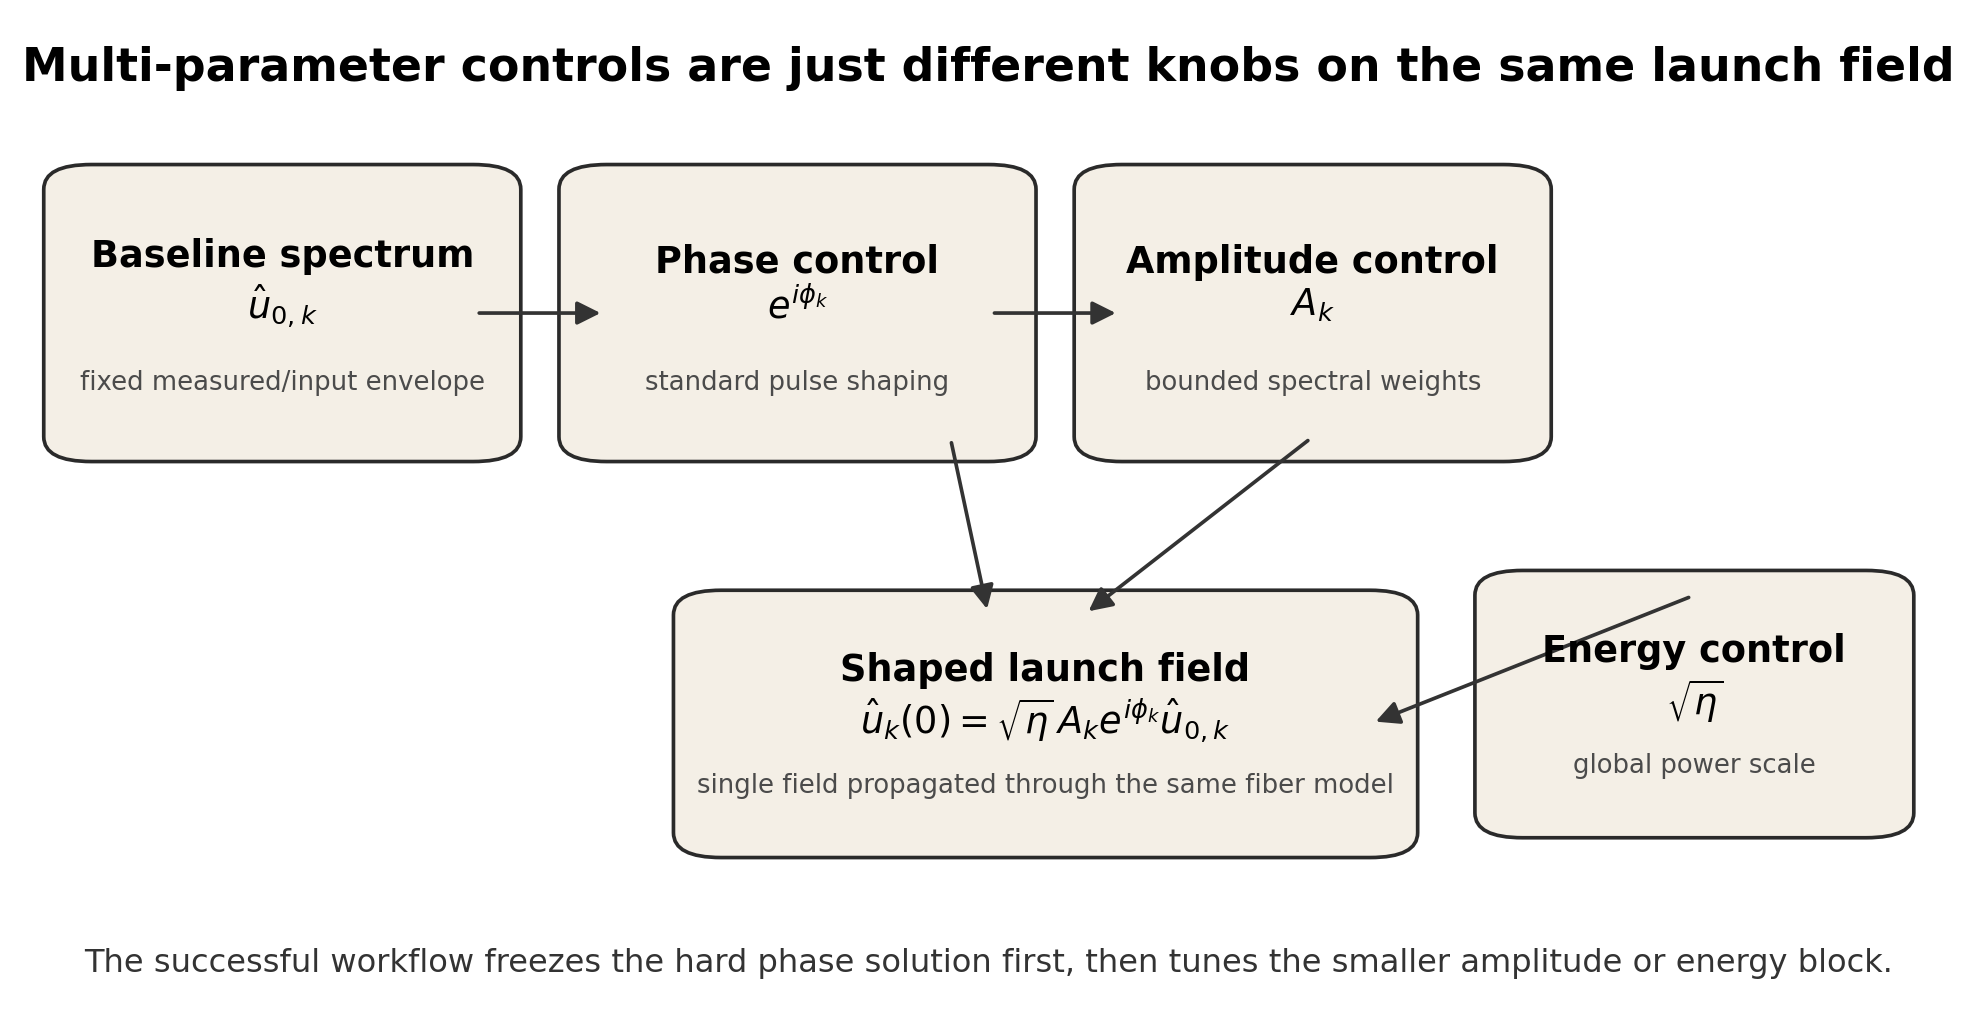
\includegraphics[width=0.95\linewidth]{figures/multivar_control_map.png}
\caption{The multi-parameter optimizer does not change the propagation model. It changes how the launch field is parameterized before the same generalized nonlinear fiber simulation is run.}
\end{figure}

\section{Model and Objective}
The propagation model is the same generalized nonlinear Schrödinger-equation family used throughout this project, with dispersion, Kerr nonlinearity, and delayed Raman response. This is the standard modeling setting described in nonlinear-fiber references such as Agrawal's \emph{Nonlinear Fiber Optics}; the numerical propagation follows the interaction-picture/RK style used in Hult's fourth-order RK4IP method for nonlinear fiber simulations.\footnote{\noteurl{https://www.sciencedirect.com/book/monograph/9780128170427/nonlinear-fiber-optics}{Agrawal, \emph{Nonlinear Fiber Optics}}; \noteurl{https://opg.optica.org/abstract.cfm?URI=JLT-25-12-3770}{Hult, ``A Fourth-Order Runge--Kutta in the Interaction Picture Method for Simulating Supercontinuum Generation in Optical Fibers.''}}

The physical Raman objective is the output spectral-energy fraction inside a Raman band $\band$:
\[
    J_{\mathrm{R}} =
    \frac{\sum_{k\in \band} |\hat u_k(L)|^2}
         {\sum_k |\hat u_k(L)|^2}.
\]
Most result tables report $10\log_{10}(J_{\mathrm{R}})$ in dB, so more negative is better. For example, $-40$ dB means the Raman-band fraction is about $10^{-4}$.

\subsection*{Regularized Surface}
The optimizer may use a regularized surface before or after dB conversion. In the runs summarized here, the relevant linear surface is
\[
    J_{\mathrm{lin}}
    =
    J_{\mathrm{R}}
    +\lambda_{\mathrm{gdd}}R_{\mathrm{gdd}}(\phi)
    +\lambda_{\mathrm{edge}}R_{\mathrm{edge}}(\phi,\Avar)
    +\lambda_E R_E(\Avar,\Escale)
    +\cdots .
\]
The energy-preservation term used for amplitude shaping is approximately
\[
    R_E =
    \left(
    \frac{\sum_k \Escale\,\Avar_k^2|\hat u_{0,k}|^2}
         {\sum_k |\hat u_{0,k}|^2}
    -1
    \right)^2.
\]
This discourages the optimizer from winning only by changing total pulse energy. It is important because amplitude shaping can change both spectral shape and total energy.

\subsection*{TL;DR for the Math}
Think of phase, amplitude, and energy as three knobs multiplying the same complex input vector. Phase rotates each frequency sample on the complex plane. Amplitude changes the radius of each sample. Energy scales the whole vector at once. The propagation code only sees the final complex vector, but the optimizer needs the chain rule telling it which knob caused which change.

\section{Gradient Chain Rules}
Let $g_k=\partial J/\partial \hat u_k(0)^*$ be the complex sensitivity of the objective with respect to the shaped input field. For
\[
    \hat u_k(0)=\sqrt{\Escale}\,\Avar_k e^{i\phi_k}\hat u_{0,k},
\]
the real gradients are
\[
    \frac{\partial J}{\partial \phi_k}
    =
    2\operatorname{Re}\left[g_k^*\,i\hat u_k(0)\right],
\]
\[
    \frac{\partial J}{\partial \Avar_k}
    =
    2\operatorname{Re}\left[
    g_k^*\,\sqrt{\Escale}e^{i\phi_k}\hat u_{0,k}
    \right],
\]
and, if the optimizer uses $\eta=\log E$ or an equivalent positive energy coordinate,
\[
    \frac{\partial J}{\partial \eta}
    =
    \operatorname{Re}\sum_k g_k^*\hat u_k(0).
\]
For multiple modes, the same formulas are summed over modes. Mode-coefficient optimization is present only as an unfinished API stub, and the current implementation strips it at runtime rather than treating it as finished.

\subsection*{Amplitude Bounds}
The current bounded amplitude parameterization is
\[
    \Avar_k = 1+\delta\tanh(\xi_k),
\]
so the physical amplitude stays inside
\[
    \Avar_k \in (1-\delta,\,1+\delta).
\]
The search variable is $\xi_k$, not $\Avar_k$ directly, so the amplitude gradient must also be multiplied by
\[
    \frac{\partial \Avar_k}{\partial \xi_k}
    =
    \delta\left(1-\tanh^2\xi_k\right).
\]
This is one reason the multi-parameter lane needed explicit gradient tests: a visually reasonable result can still be wrong if this chain rule is missing.

\subsection*{Boundary Regularizer Correction}
The temporal-edge regularizer is a fraction,
\[
    R_{\mathrm{edge}}=
    \frac{\sum_j w_j |u(t_j,0)|^2}{\sum_j |u(t_j,0)|^2}.
\]
For phase-only perturbations the denominator is effectively fixed, but amplitude changes alter both numerator and denominator. The corrected amplitude derivative therefore uses the quotient rule, not only the edge numerator. This correction is now covered by the multivariable gradient smoke test.

\subsection*{TL;DR for Explaining the Derivatives}
If someone asks why the amplitude derivative is different from the phase derivative, use the complex-plane picture. Phase pushes each spectral sample tangent to its circle, because $d(e^{i\phi})/d\phi=i e^{i\phi}$. Amplitude pushes it radially outward or inward. Energy pushes every sample radially together. The adjoint tells us which push would most reduce Raman leakage.

\section{Implementation Surface}
\begingroup
\footnotesize
\begin{tabularx}{\linewidth}{@{}p{0.32\linewidth}X@{}}
\toprule
\textbf{File or directory} & \textbf{Role in this lane} \\
\midrule
\nolinkurl{scripts/research/multivar/multivar_optimization.jl} & Core cost, gradient, variable packing, amplitude bounds, regularizers, and result serialization. \\
\nolinkurl{scripts/research/multivar/multivar_amp_on_phase_ablation.jl} & Runs the two-stage amplitude-on-fixed-phase ablation. This is the most important current workflow. \\
\nolinkurl{scripts/research/multivar/multivar_variable_ablation.jl} & Runs variable-combination studies: amplitude-only, energy-only, amplitude+energy, and warm joint variants. \\
\nolinkurl{scripts/workflows/refine_amp_on_phase.jl} & User-facing wrapper for the optional two-stage refinement workflow. Supports dry-run, export, and amplitude-bound options. \\
\nolinkurl{scripts/canonical/refine_amp_on_phase.jl} & Thin canonical entry point that calls the workflow wrapper. \\
\nolinkurl{scripts/canonical/export_run.jl} & Exports amplitude-aware handoff bundles after a successful refinement run. \\
\nolinkurl{scripts/dev/smoke/test_multivar_unit.jl} & Checks variable sanitation, packing/unpacking, scaling, and config defaults. \\
\nolinkurl{scripts/dev/smoke/test_multivar_gradients.jl} & Checks finite-difference agreement for phase, amplitude, energy, mixed-variable gradients, and save/load behavior. \\
\bottomrule
\end{tabularx}
\endgroup

\section{Experimental Strategy}
\begin{figure}[H]
\centering
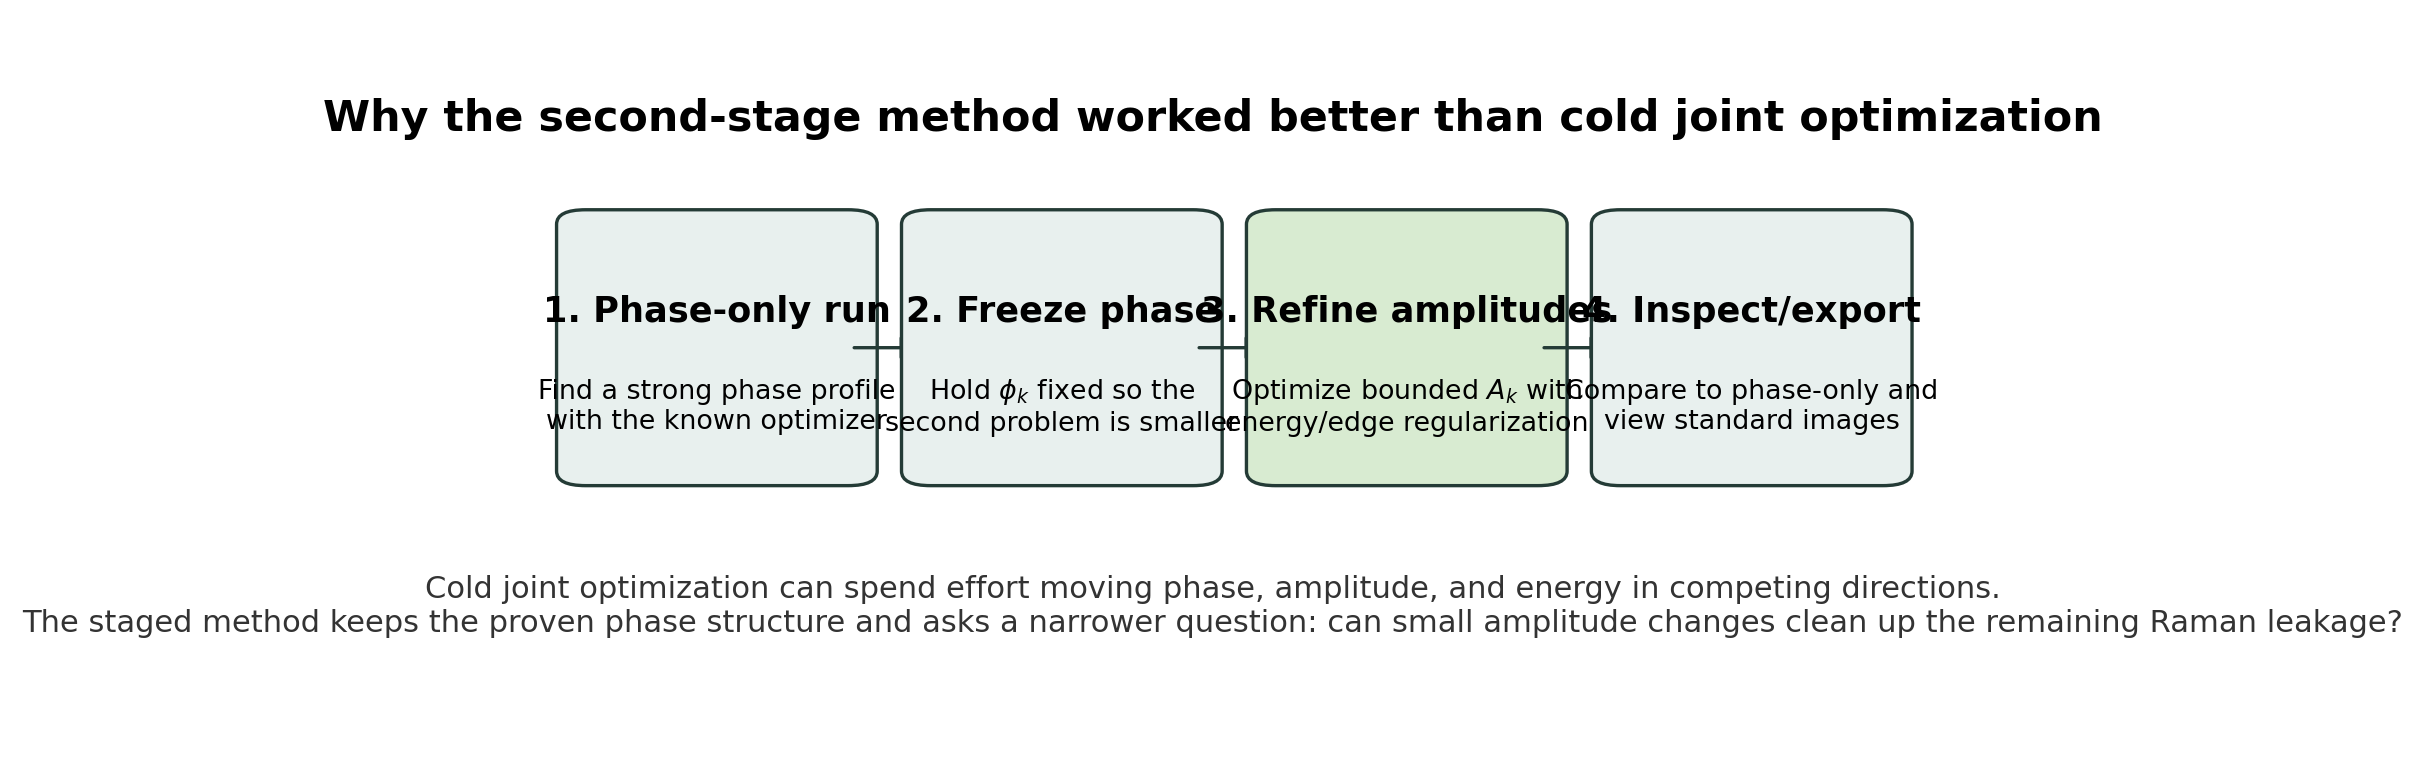
\includegraphics[width=0.95\linewidth]{figures/two_stage_workflow.png}
\caption{The staged workflow is intentionally less ambitious than full joint optimization. It first solves the hard phase problem, then asks whether a smaller amplitude or energy correction can clean up the remaining Raman leakage.}
\end{figure}

The experiments followed four ladders:
\begin{enumerate}
    \item \textbf{No-shaping control.} Propagate the input pulse with flat phase and unit amplitude.
    \item \textbf{Phase-only reference.} Use the established phase optimizer at the same fiber and power point.
    \item \textbf{Broad joint search.} Optimize phase and amplitude together from cold and warm starts. This tested the original ``more knobs should help'' hypothesis.
    \item \textbf{Fixed-phase refinement.} Freeze the phase-only solution and optimize amplitude, energy, or amplitude+energy on top of it.
\end{enumerate}

The canonical point is SMF-28, $L=2.0$ m, $P=0.30$ W, with the same pulse and Raman-band conventions as the surrounding project notes. Stronger local checks varied length and power near that point.

\section{Representative Results}
\subsection{Control Group}
\begin{figure}[H]
\centering
\begin{minipage}{0.48\linewidth}
\centering
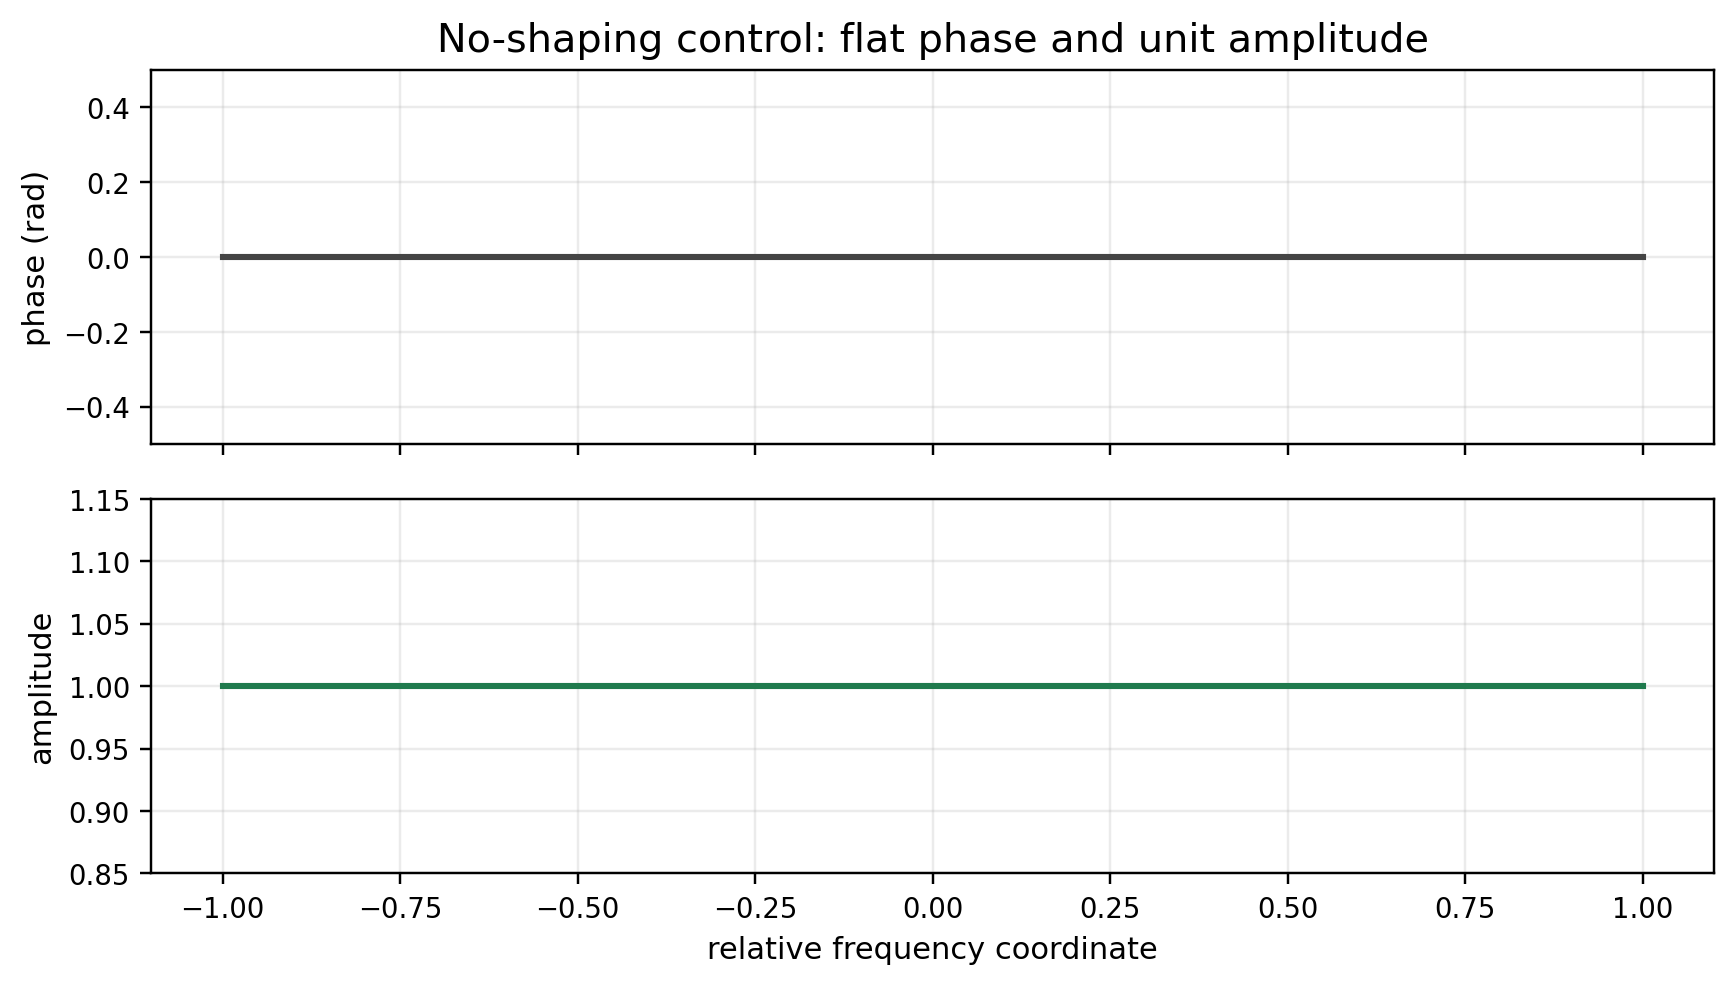
\includegraphics[width=\linewidth]{figures/no_shaping_control_profile.png}
\caption*{No-shaping input: flat phase and unit amplitude.}
\end{minipage}
\hfill
\begin{minipage}{0.48\linewidth}
\centering
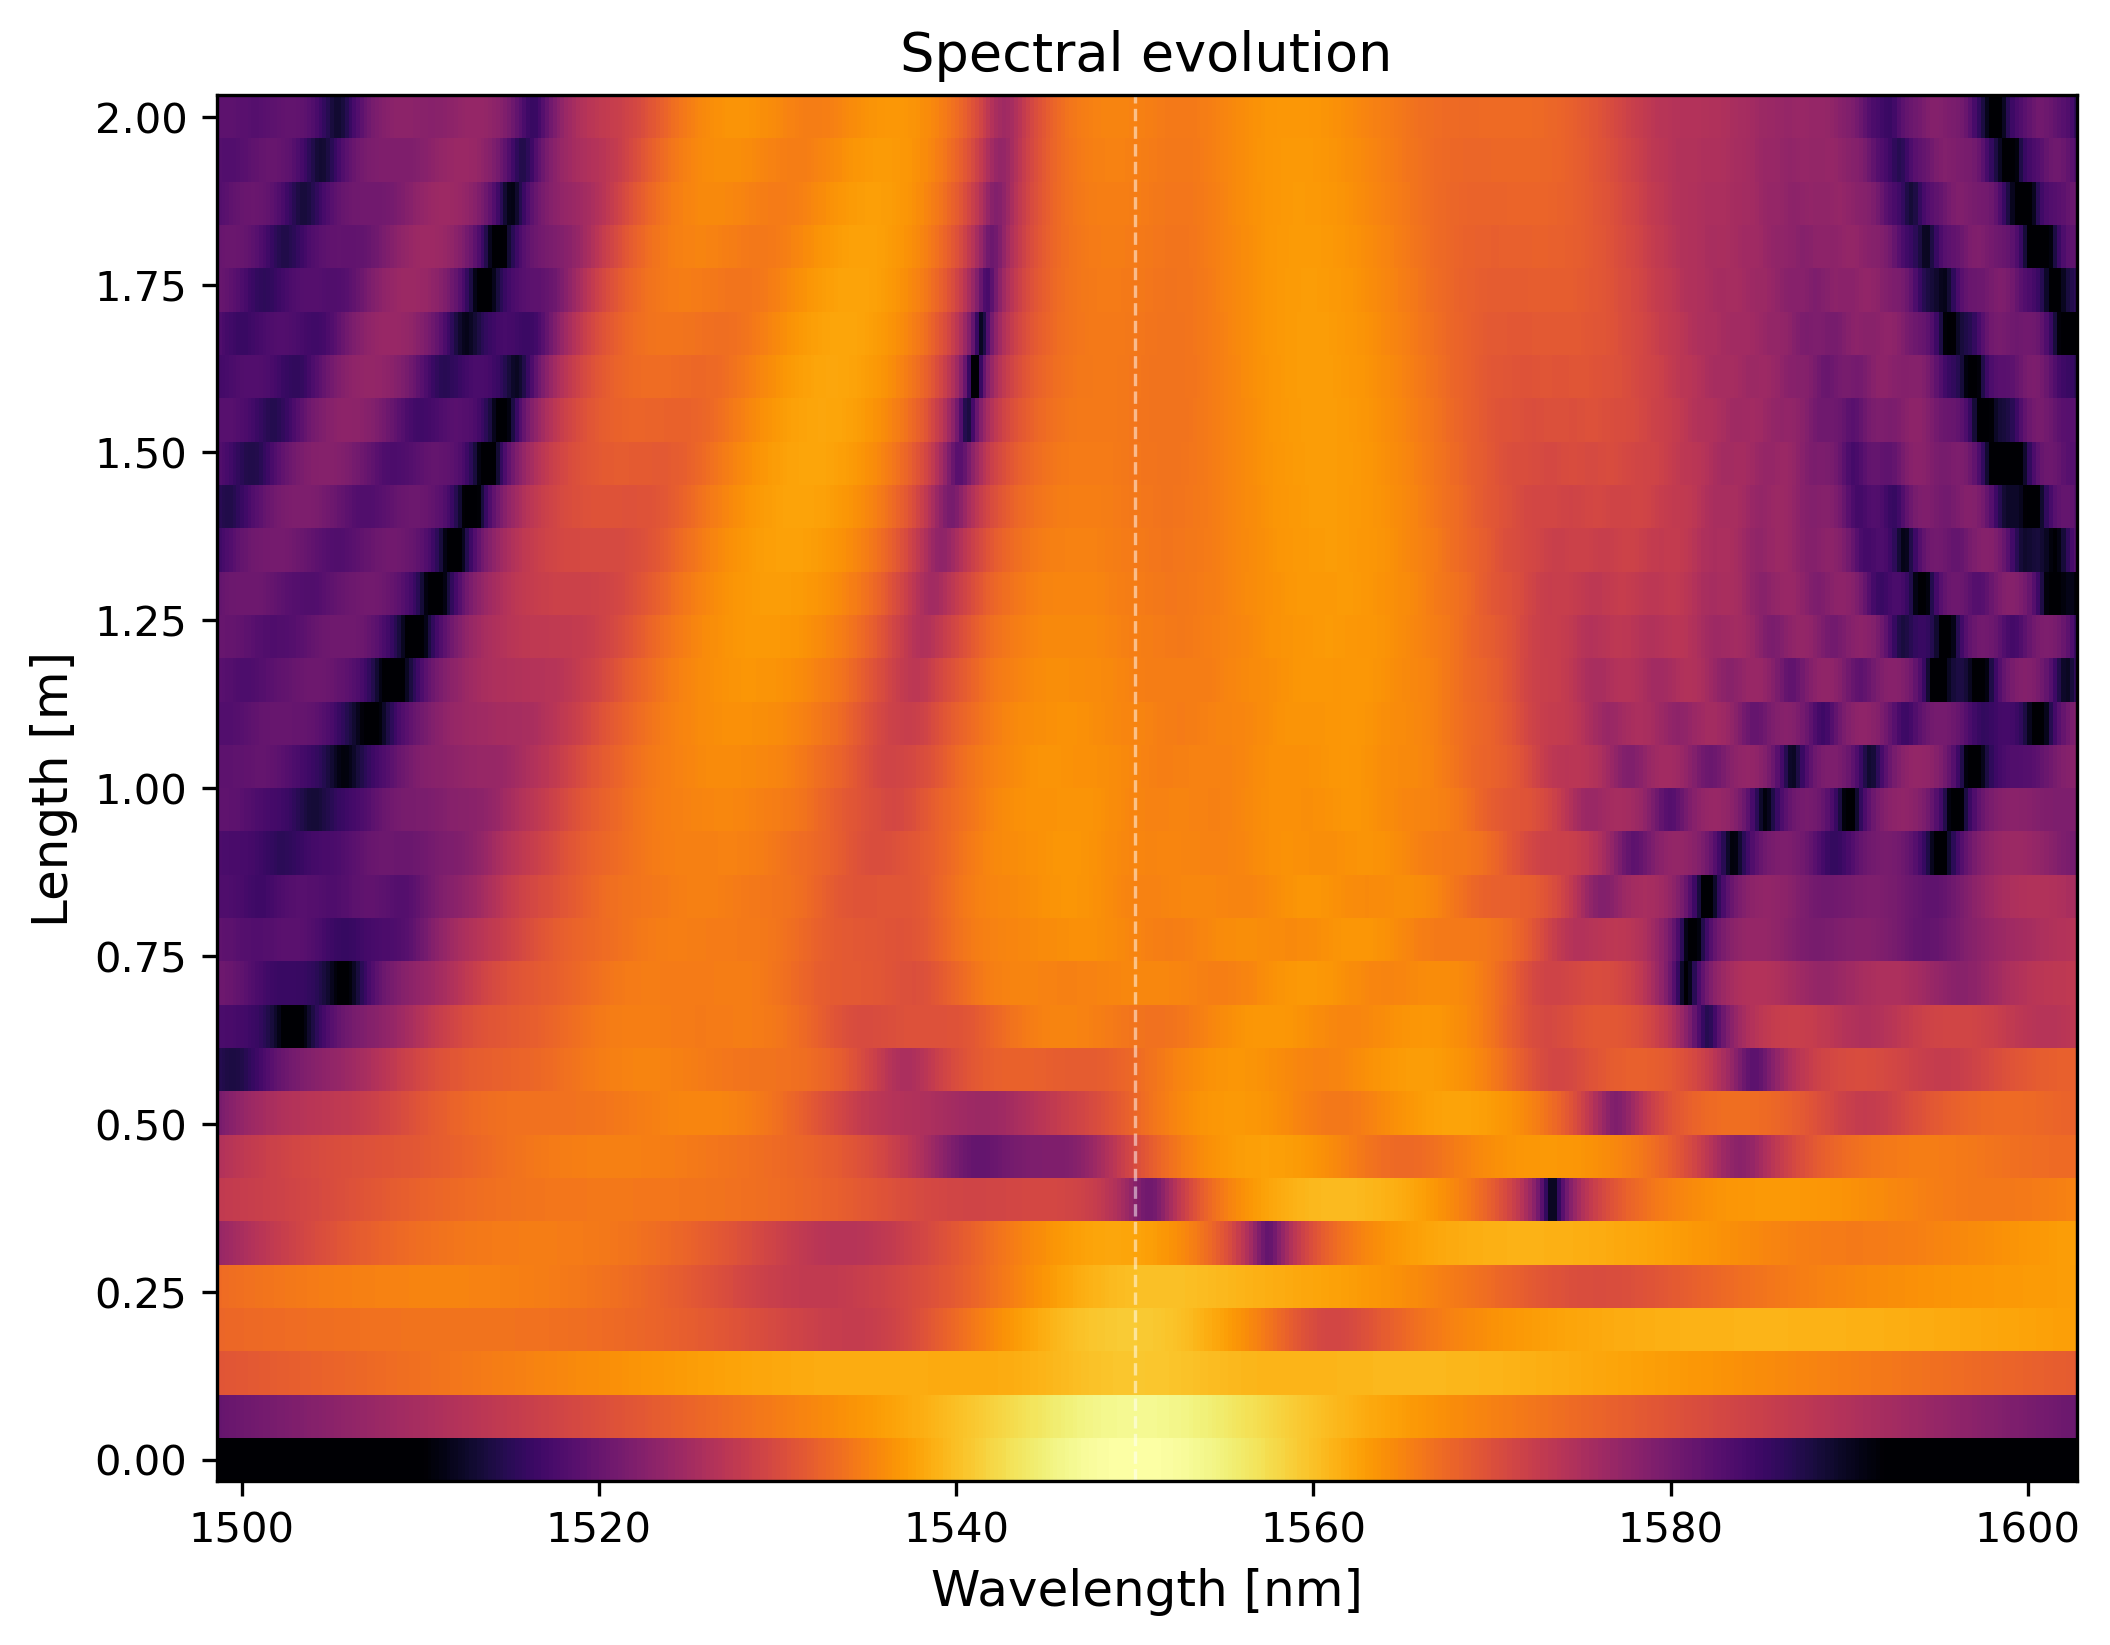
\includegraphics[width=\linewidth]{figures/no_shaping_control_evolution.png}
\caption*{No-shaping propagation heatmap.}
\end{minipage}
\caption{The control group is the reference for asking whether shaping is doing real work. It should not be confused with the phase-only reference, which is already optimized.}
\end{figure}

\subsection{Phase-Only Reference}
\begin{figure}[H]
\centering
\begin{minipage}{0.48\linewidth}
\centering
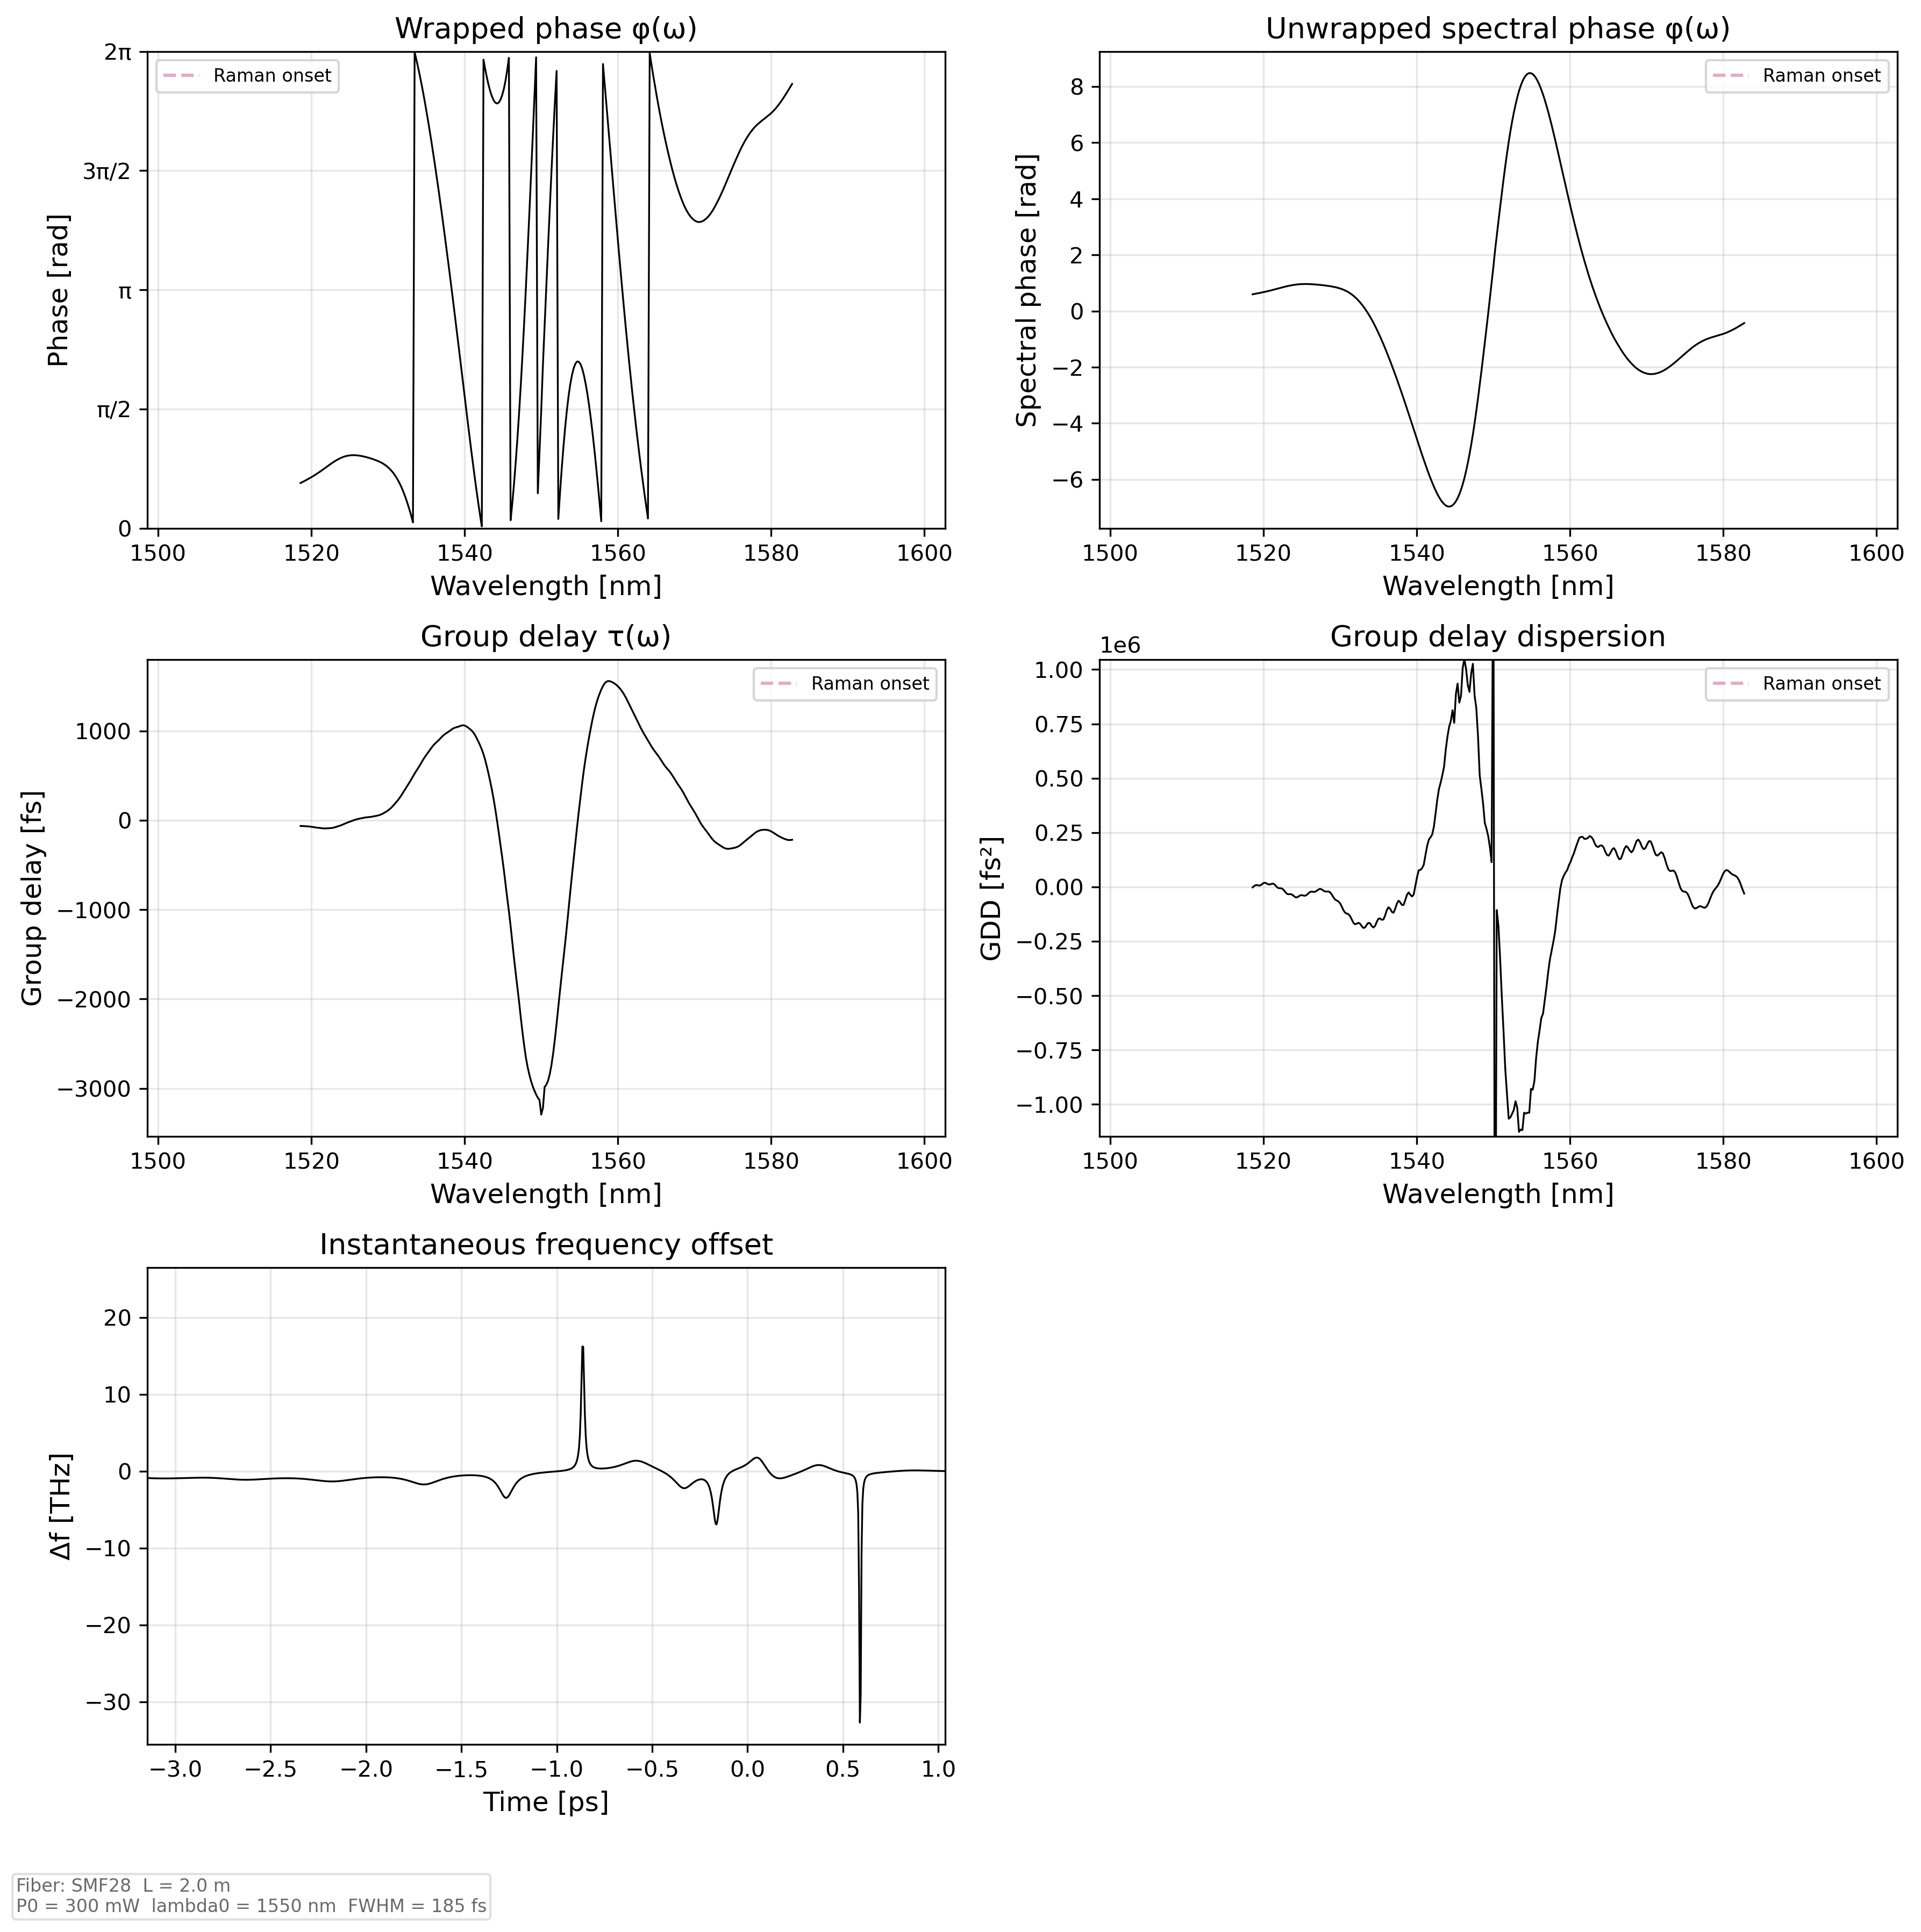
\includegraphics[width=\linewidth]{figures/phase_only_reference_phase_diagnostic.png}
\caption*{Phase-only diagnostic.}
\end{minipage}
\hfill
\begin{minipage}{0.48\linewidth}
\centering
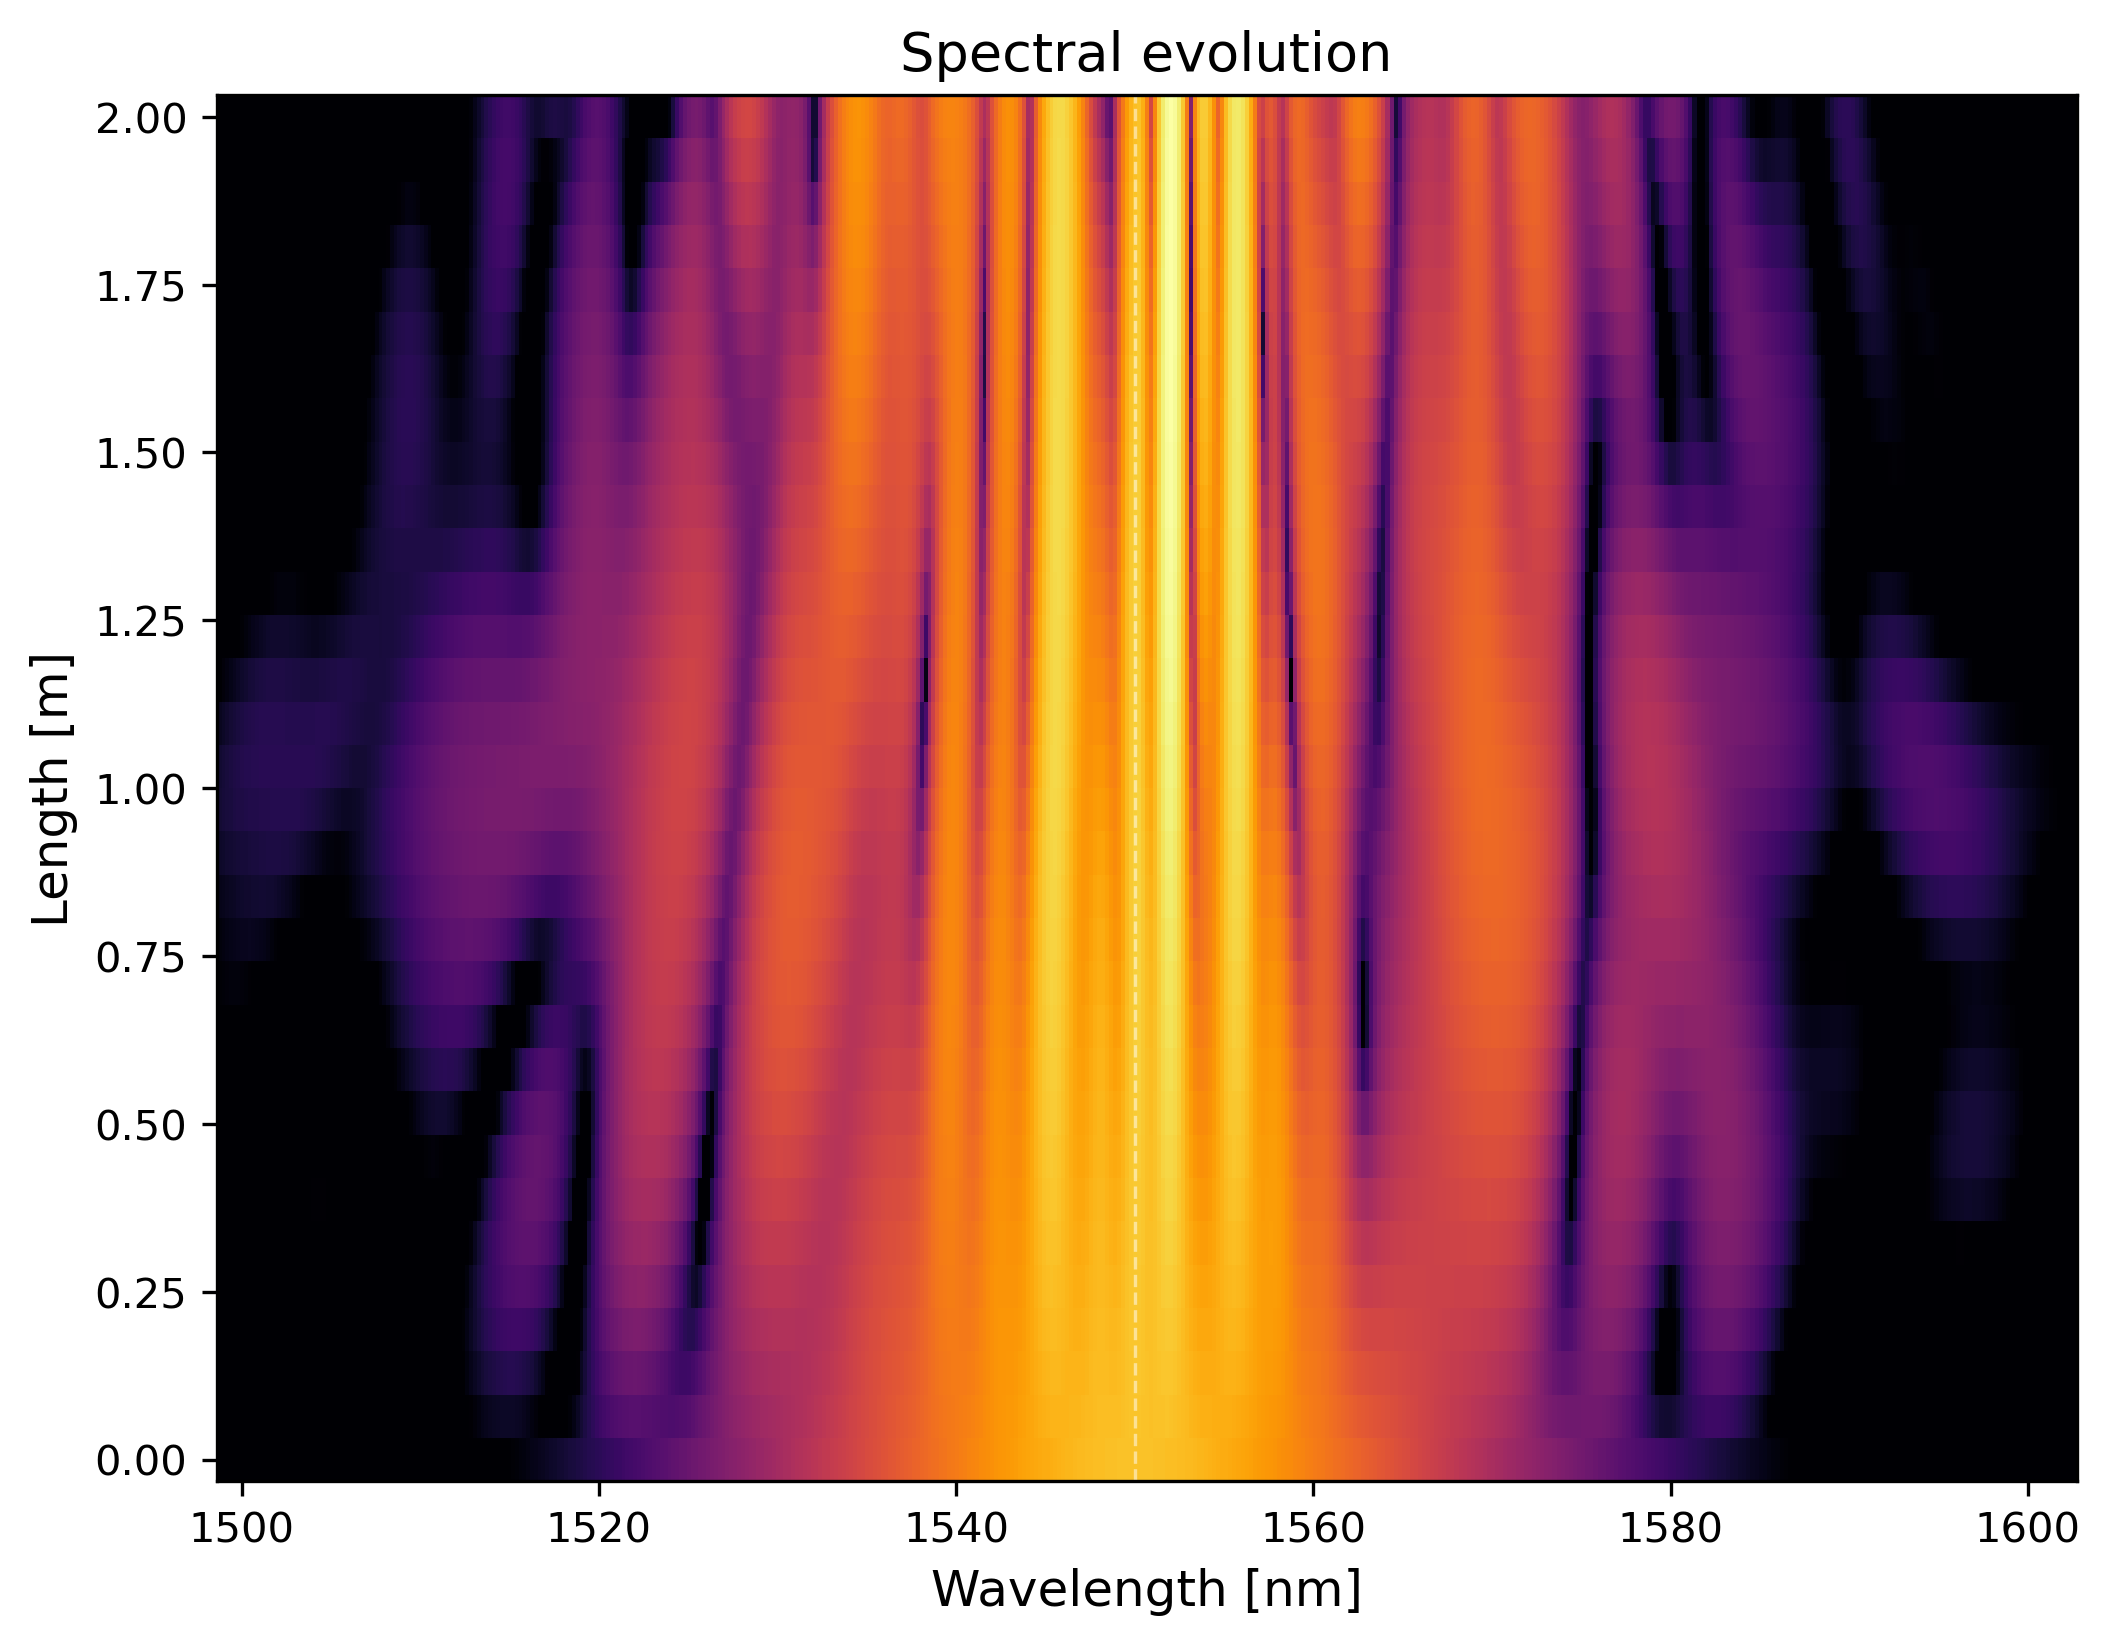
\includegraphics[width=\linewidth]{figures/phase_only_reference_evolution.png}
\caption*{Phase-only propagation heatmap.}
\end{minipage}
\caption{The phase-only run is the baseline the multivariable methods must beat. At the canonical point it reached $J_{\mathrm{R}}=-40.79$ dB.}
\end{figure}

\subsection{Amplitude-On-Phase Refinement}
\begin{figure}[H]
\centering
\begin{minipage}{0.48\linewidth}
\centering
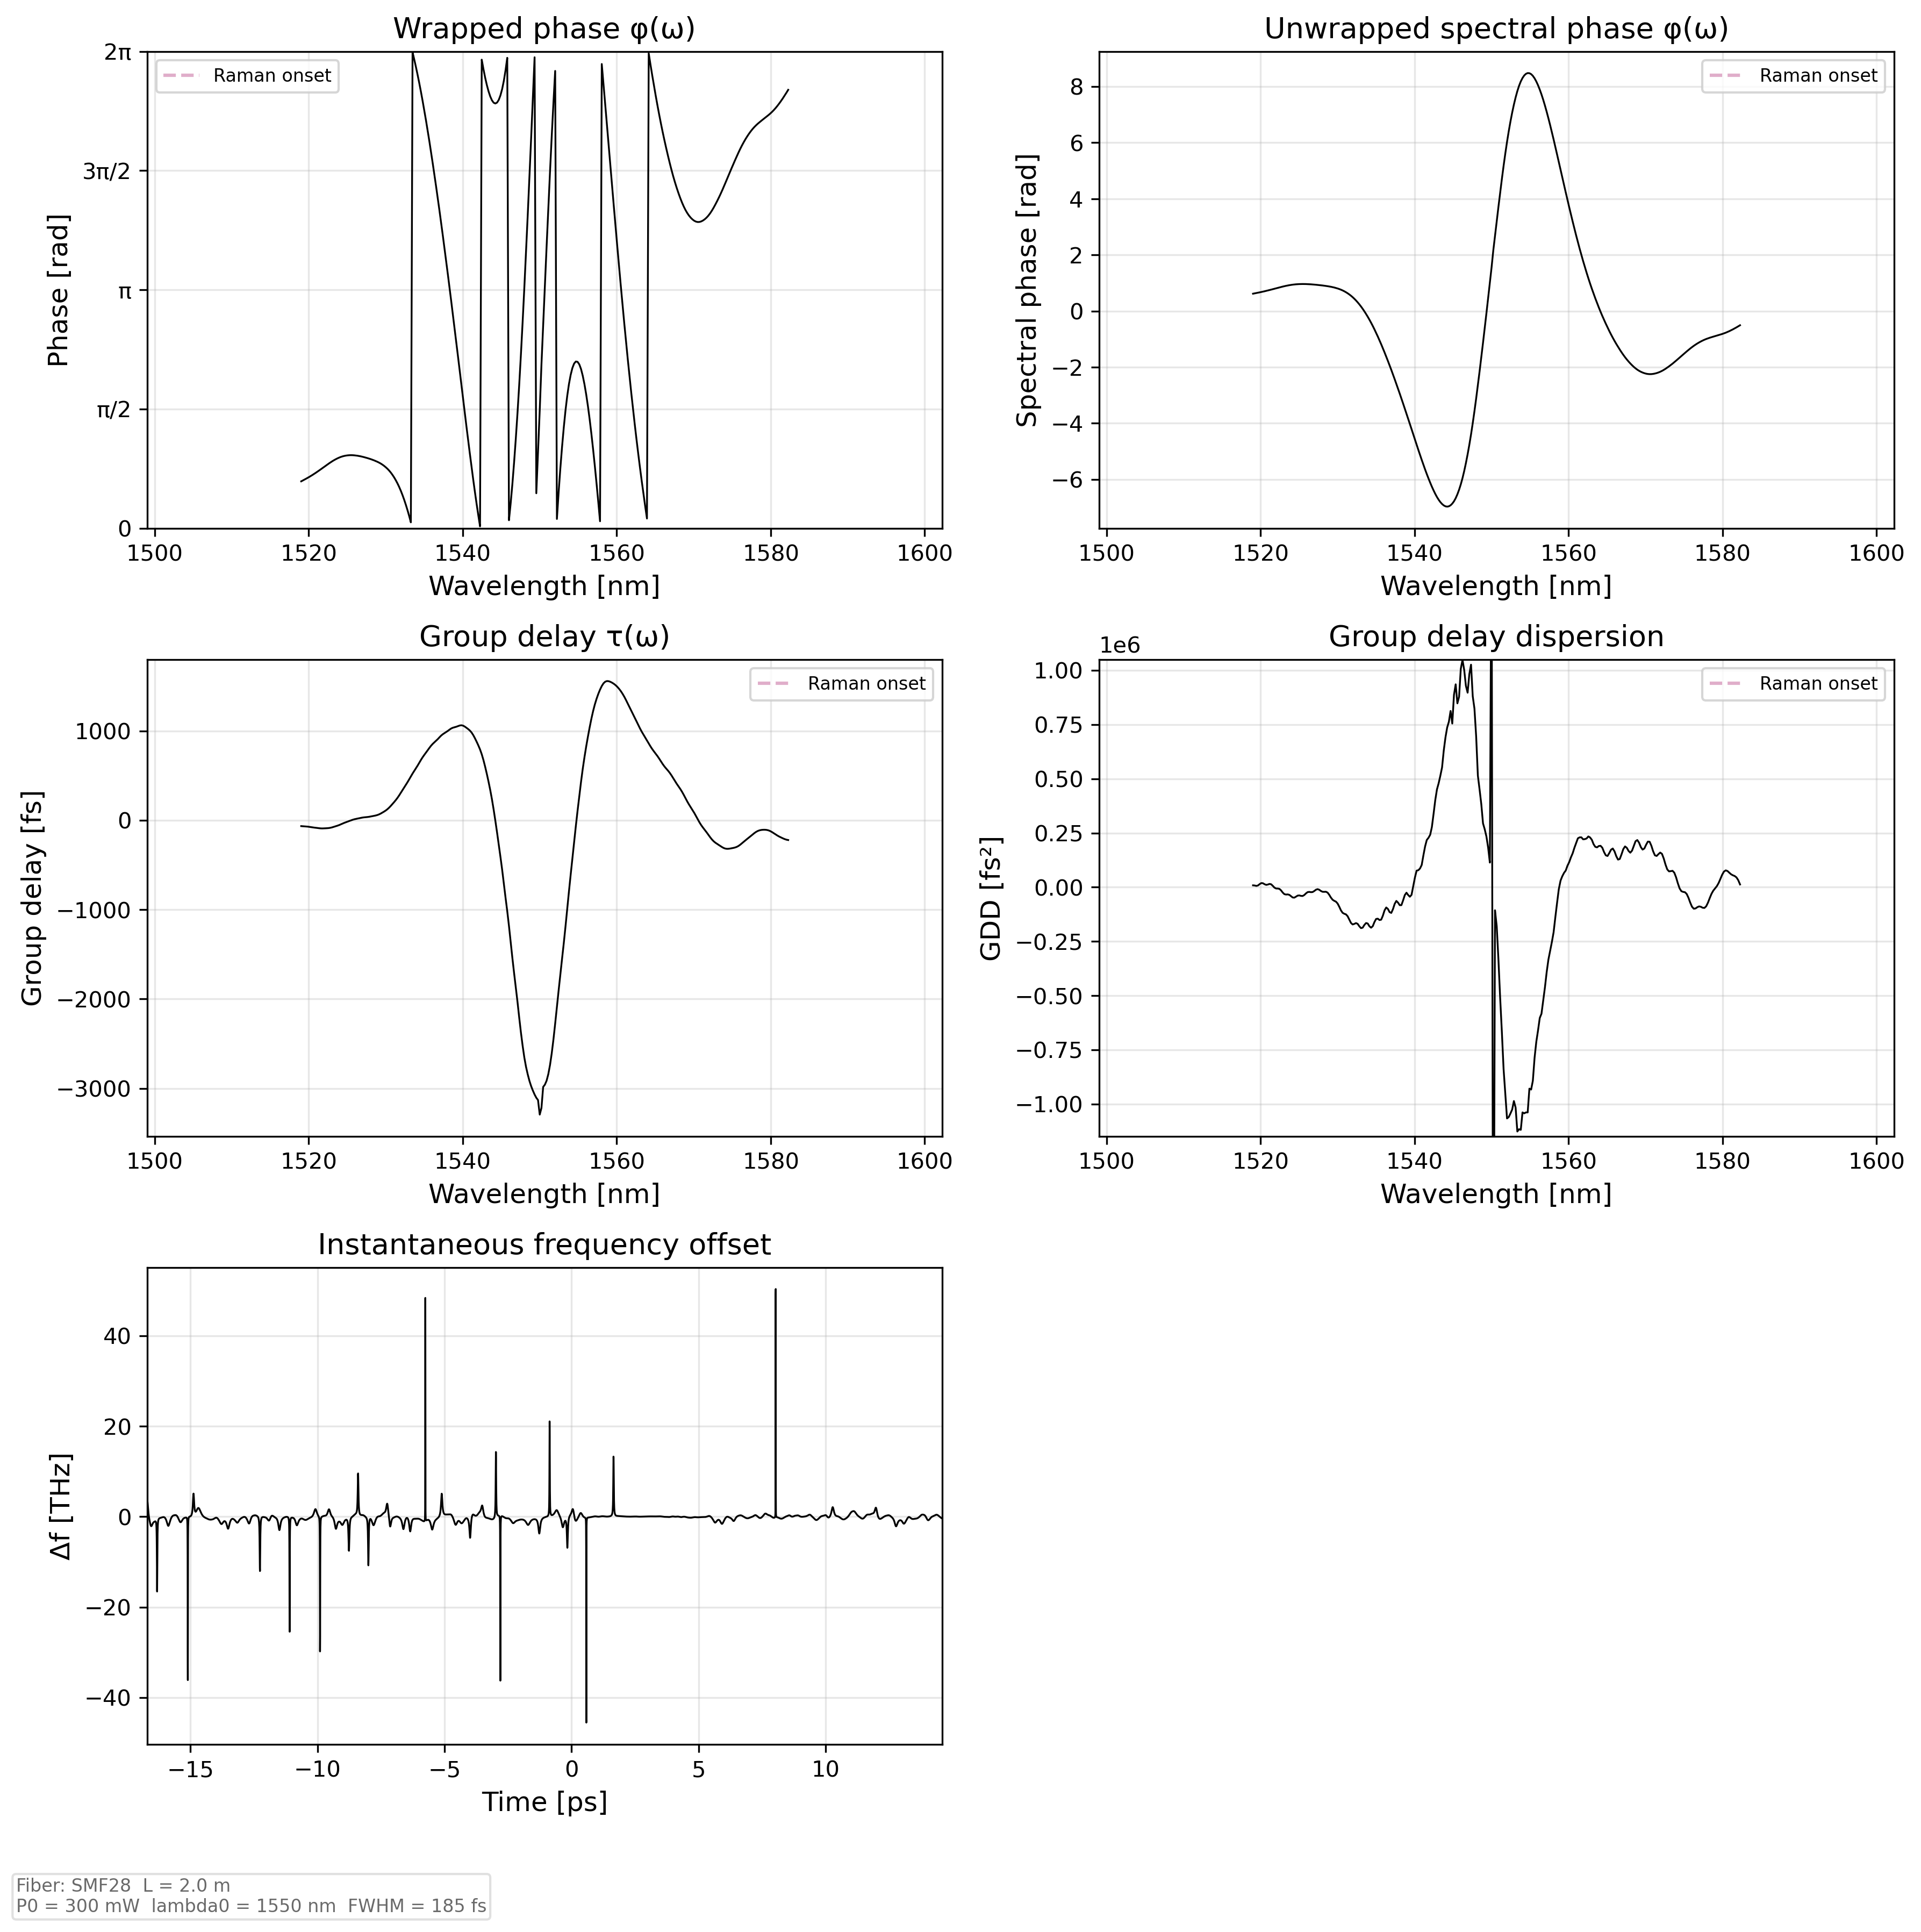
\includegraphics[width=\linewidth]{figures/amplitude_refinement_phase_diagnostic.png}
\caption*{Amplitude-refined diagnostic.}
\end{minipage}
\hfill
\begin{minipage}{0.48\linewidth}
\centering
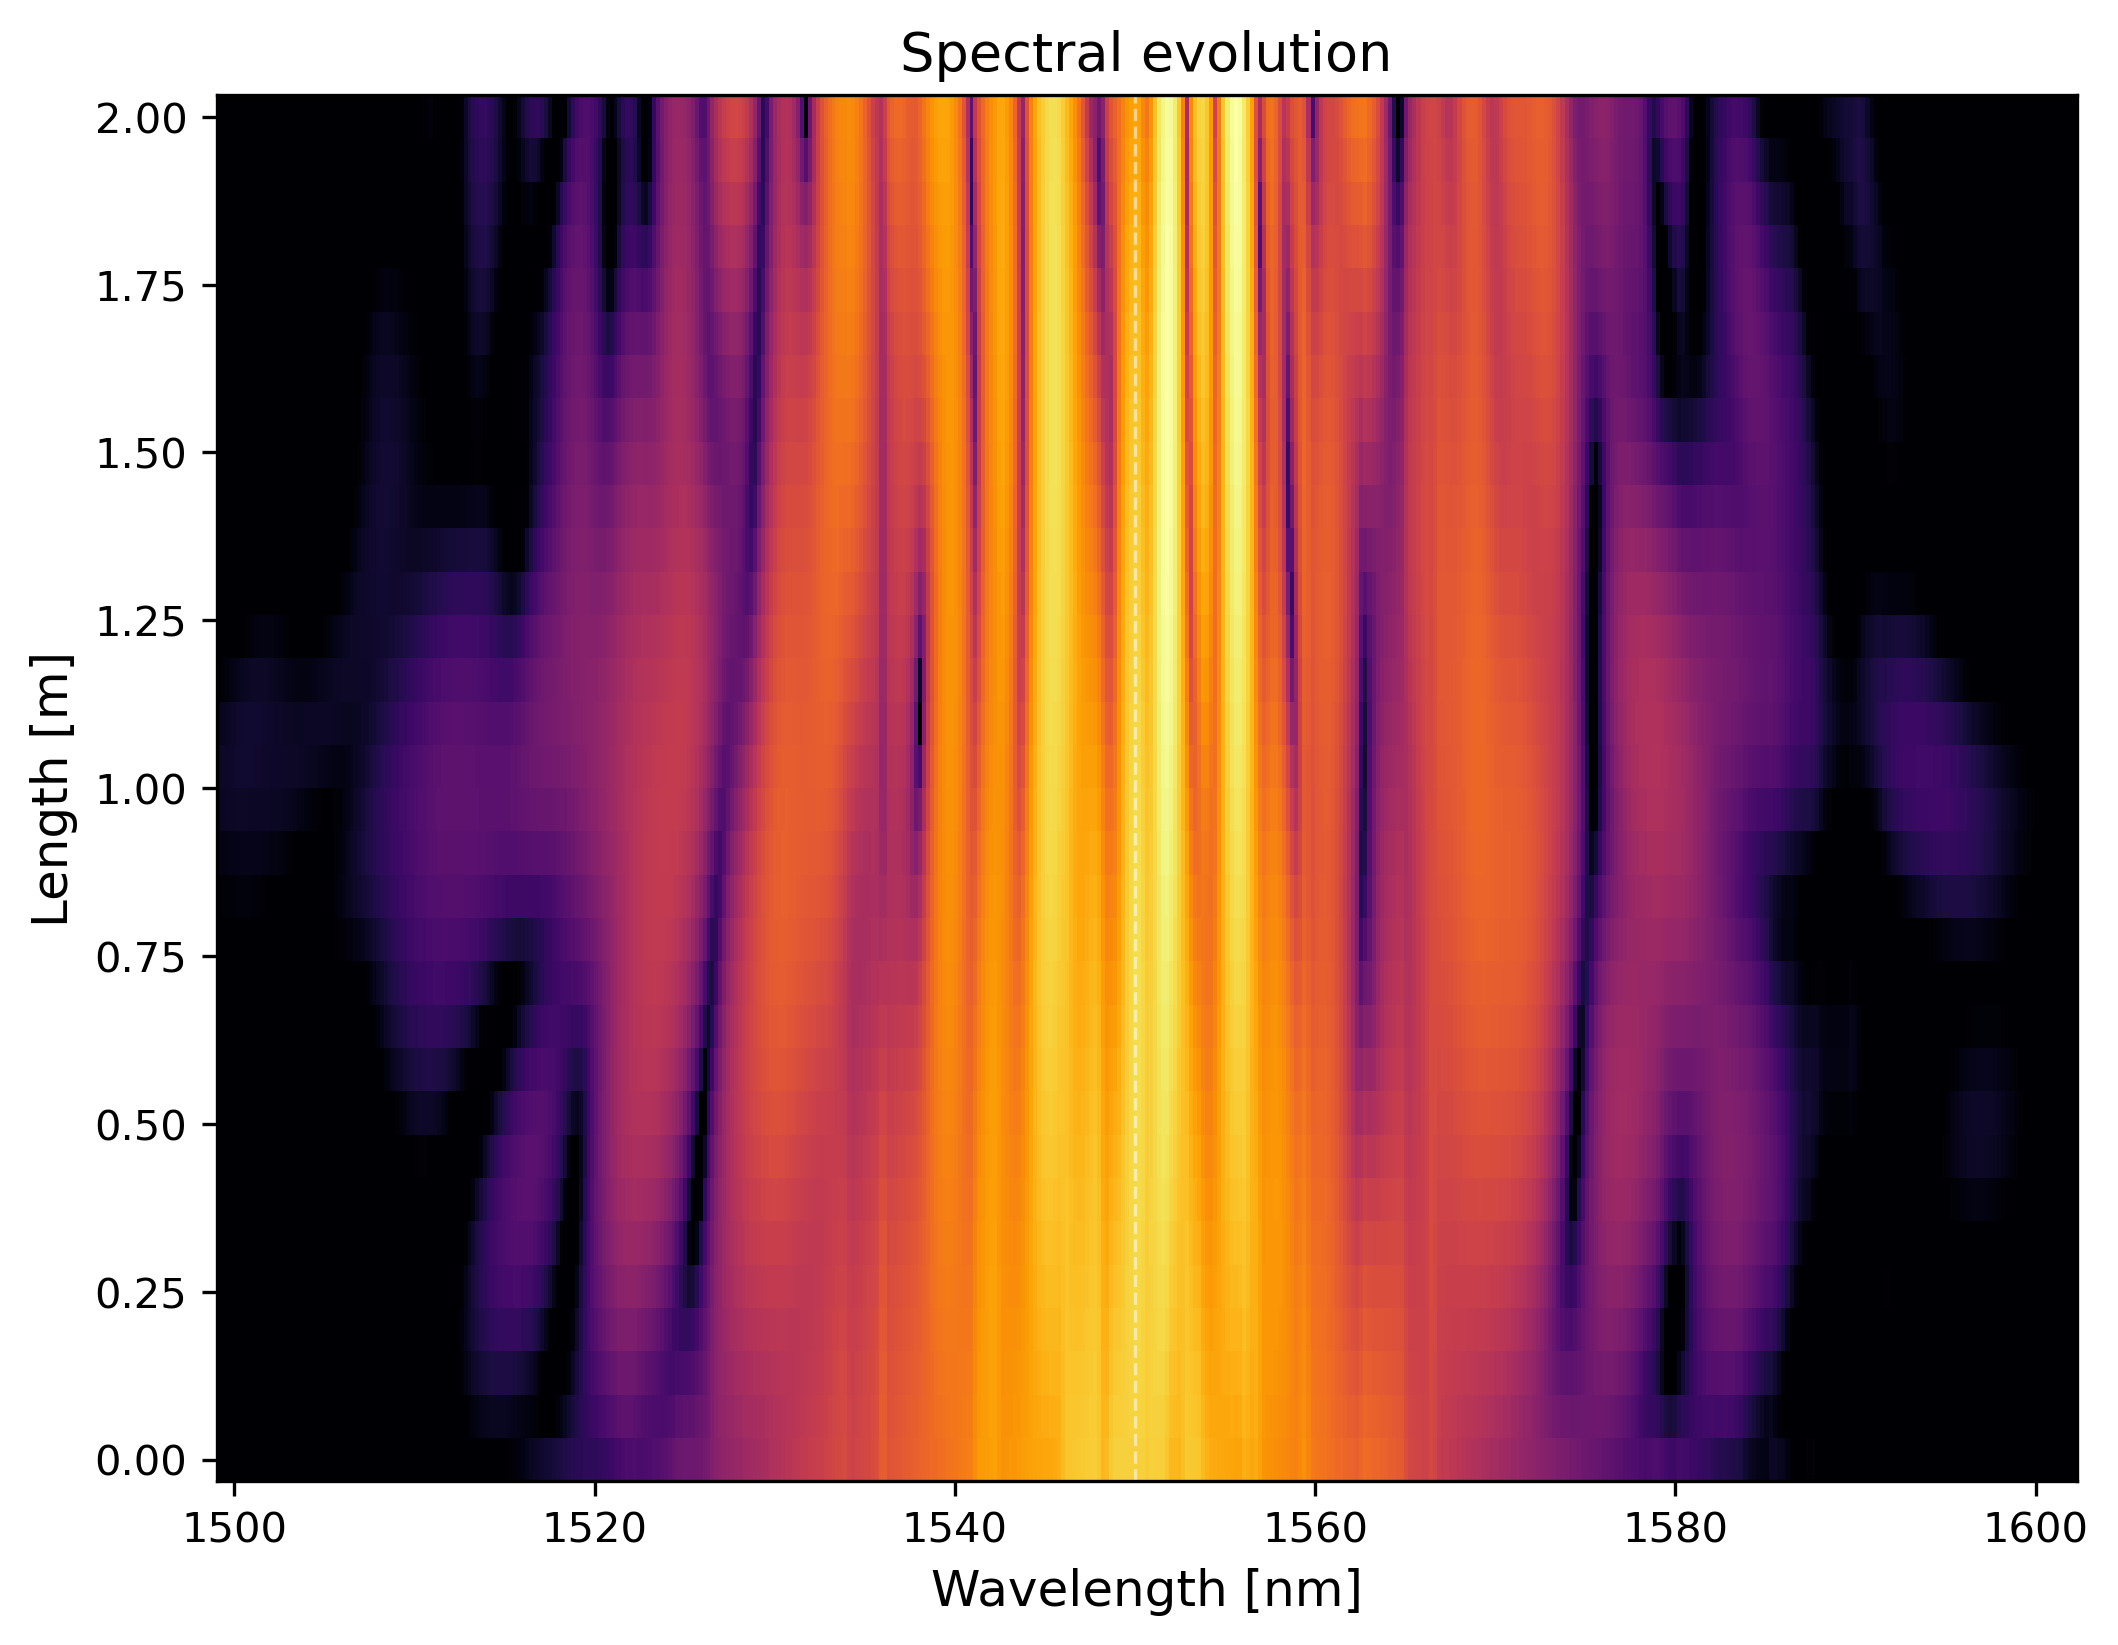
\includegraphics[width=\linewidth]{figures/amplitude_refinement_evolution.png}
\caption*{Amplitude-refined propagation heatmap.}
\end{minipage}
\caption{The strongest canonical amplitude-on-fixed-phase ablation reached $J_{\mathrm{R}}=-46.91$ dB, improving the phase-only reference by $6.12$ dB. This run hit the 50-iteration cap, so the value should be read as a strong simulated result rather than a fully converged final optimum.}
\end{figure}

\subsection{Energy-On-Phase Refinement}
\begin{figure}[H]
\centering
\begin{minipage}{0.48\linewidth}
\centering
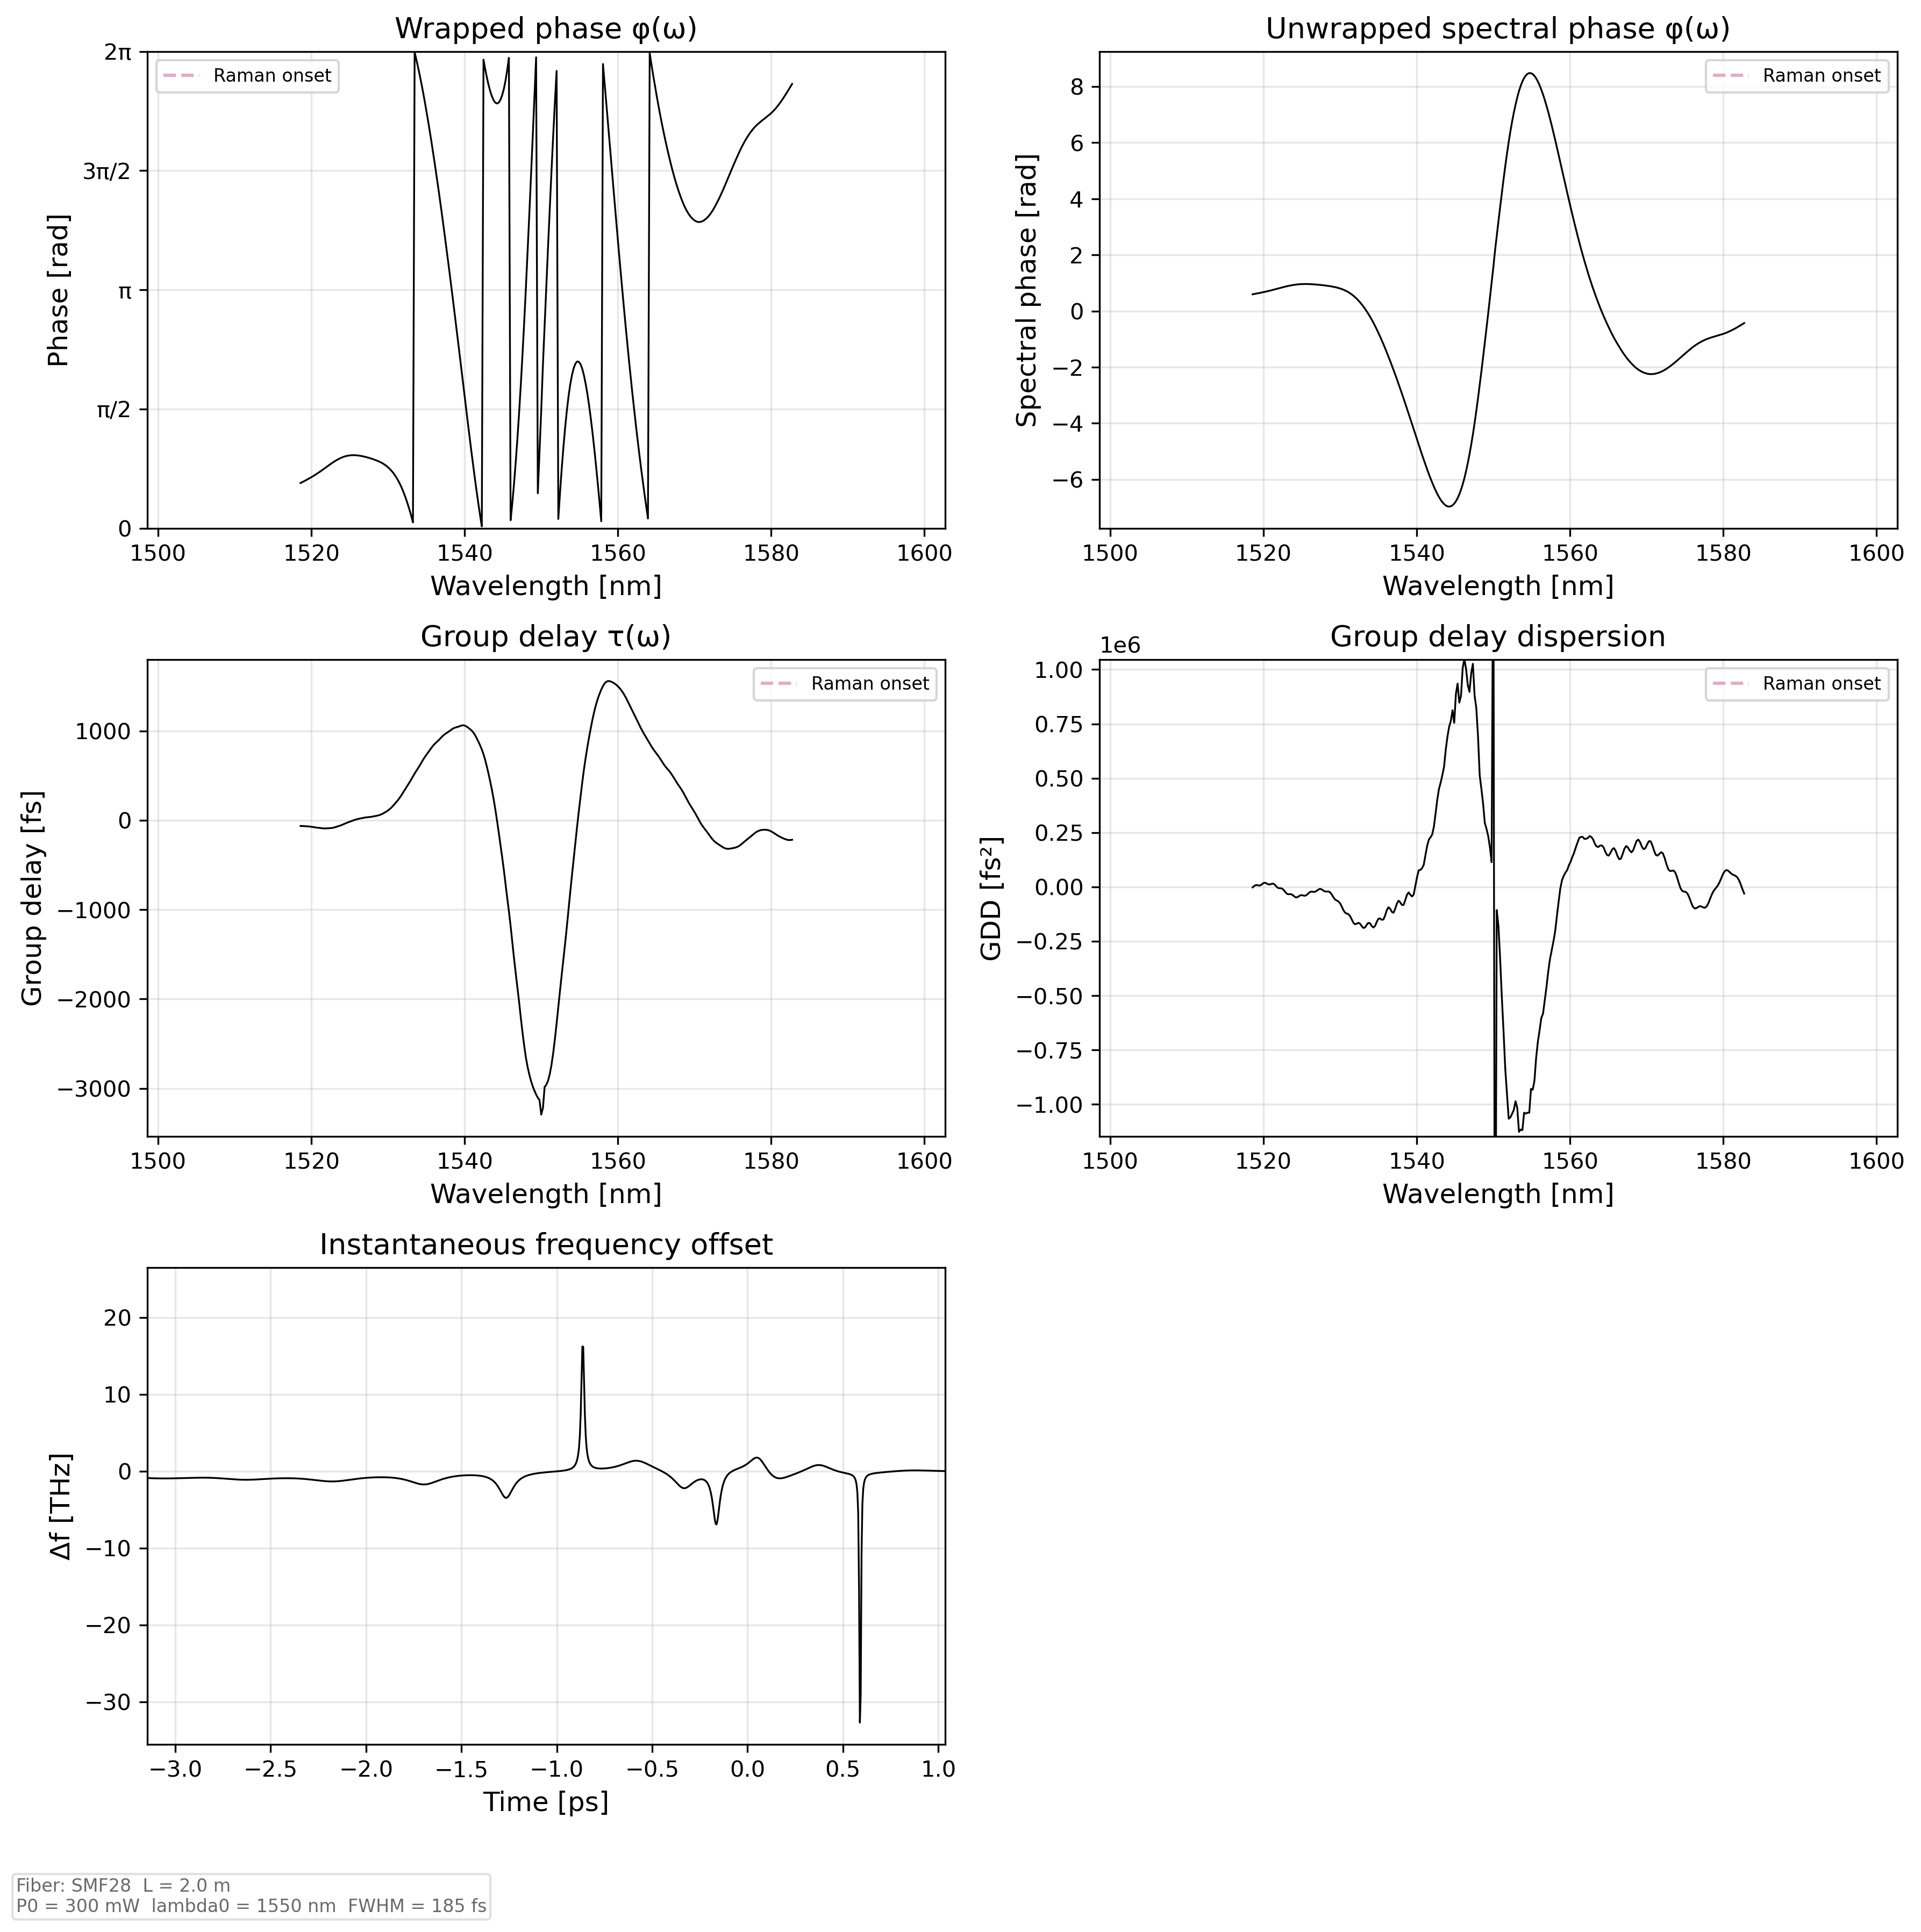
\includegraphics[width=\linewidth]{figures/energy_refinement_phase_diagnostic.png}
\caption*{Energy-refined diagnostic.}
\end{minipage}
\hfill
\begin{minipage}{0.48\linewidth}
\centering
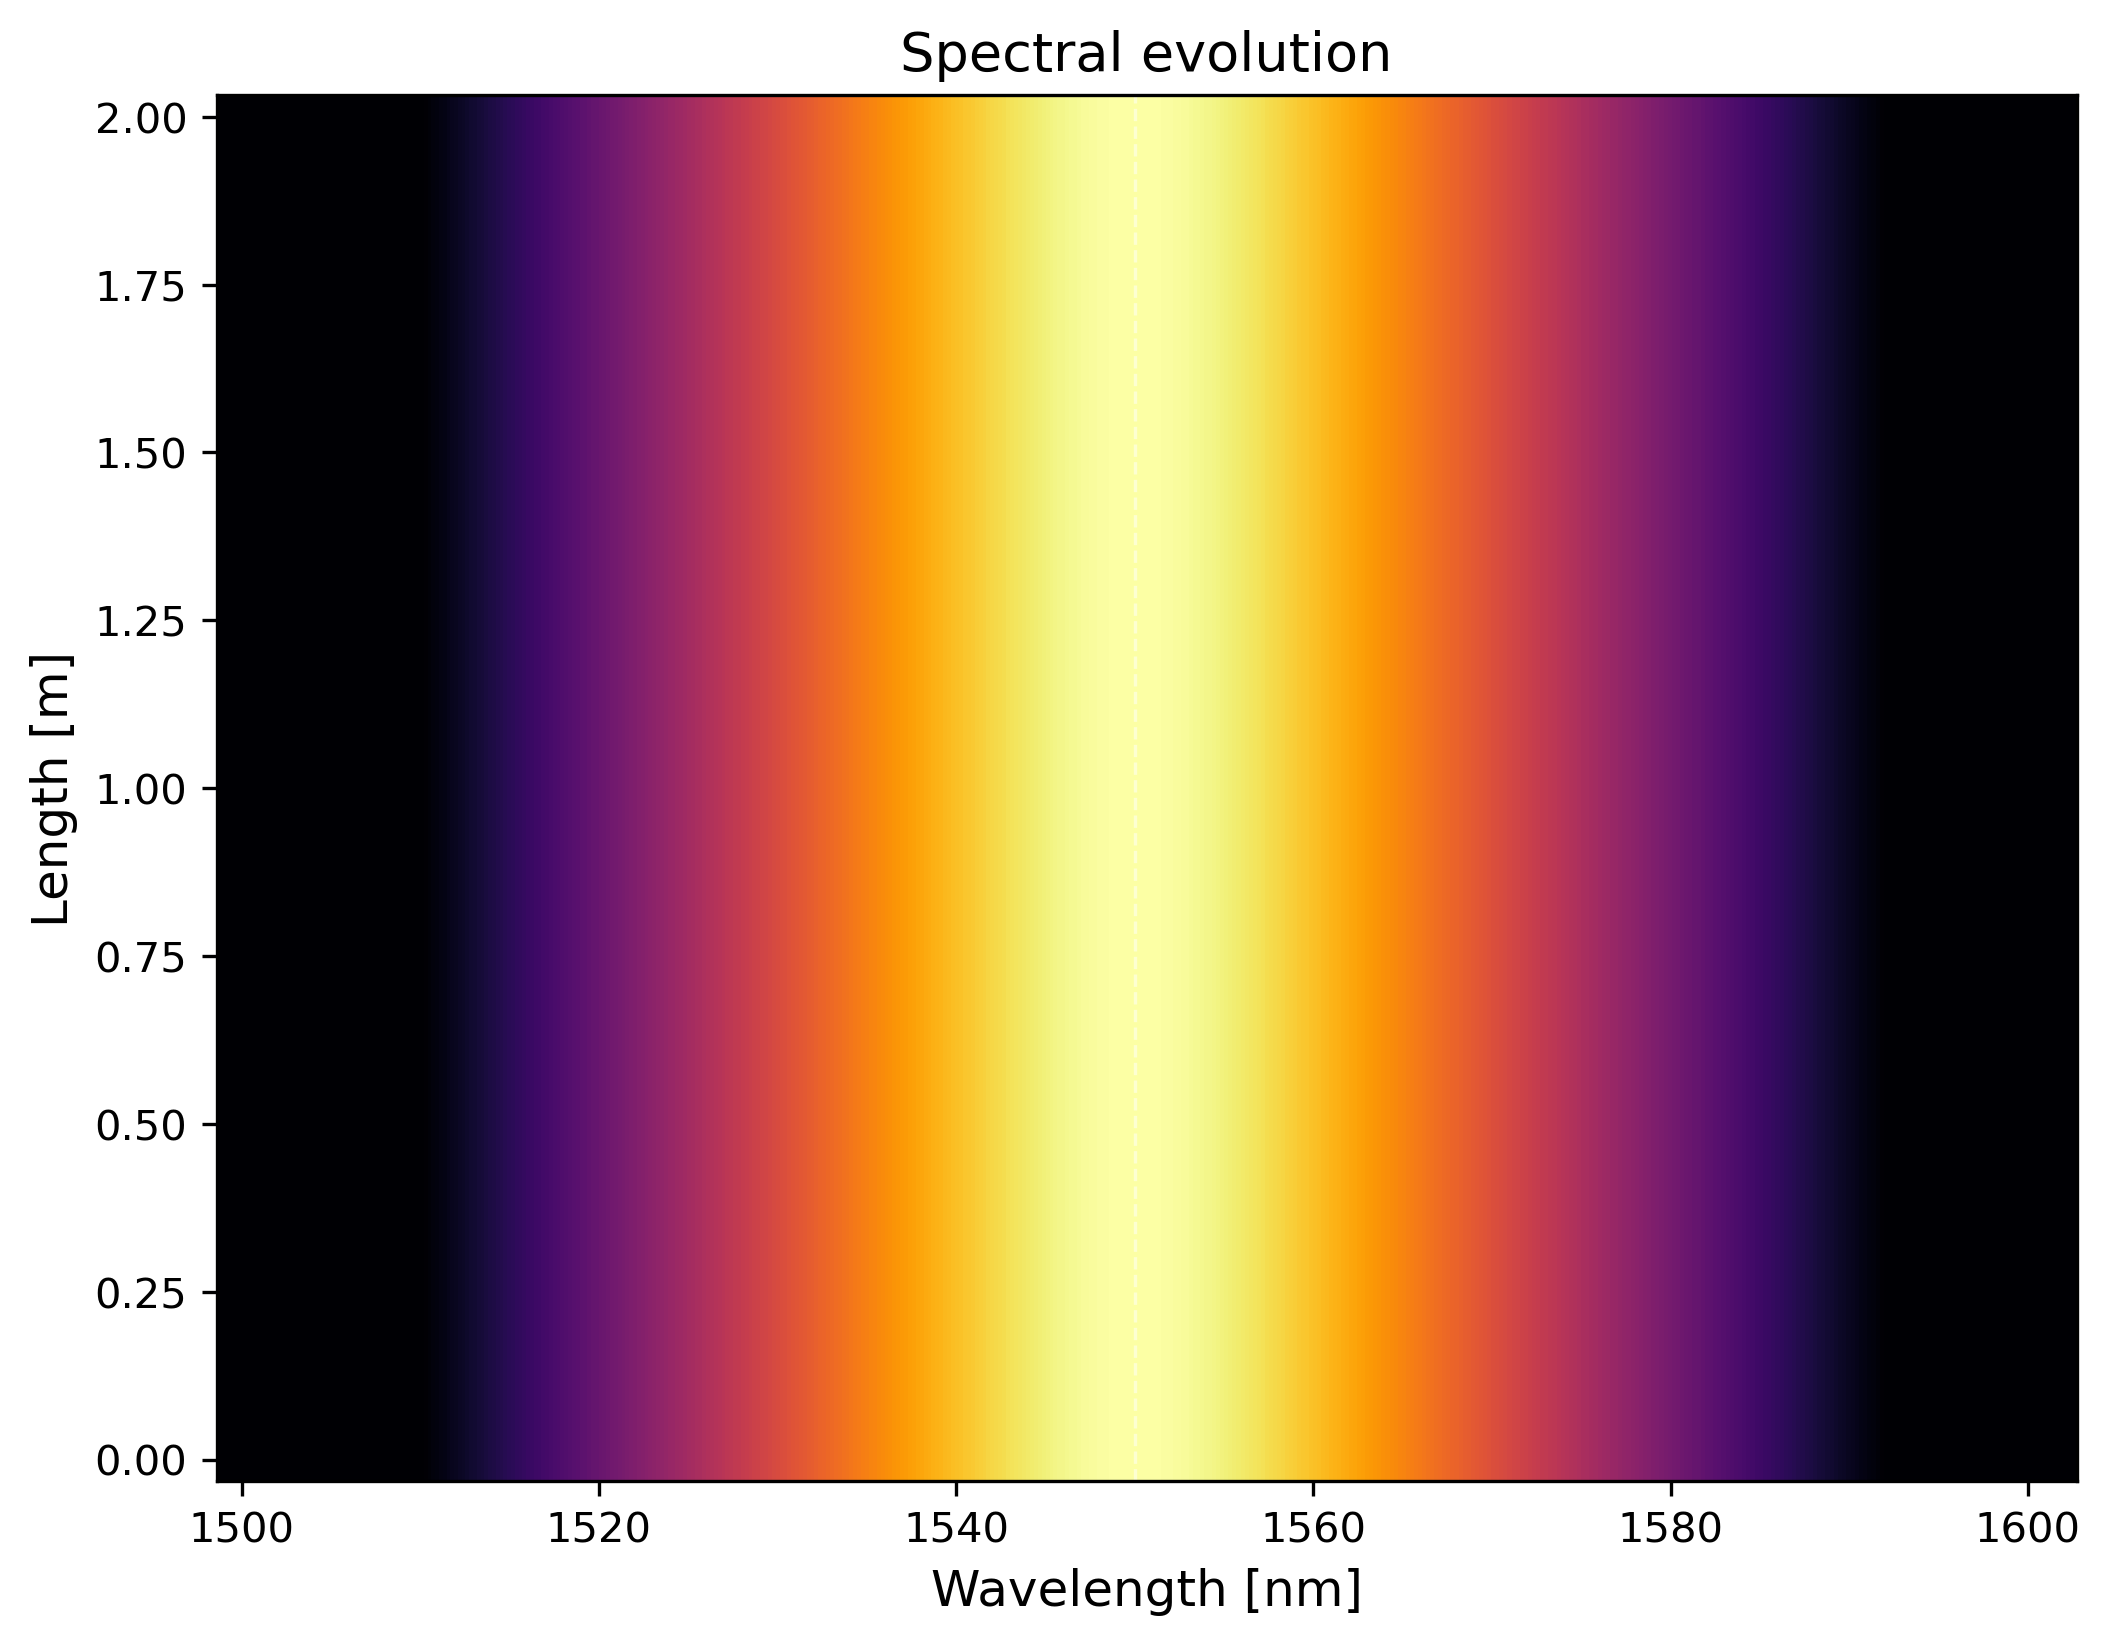
\includegraphics[width=\linewidth]{figures/energy_refinement_evolution.png}
\caption*{Energy-refined propagation heatmap.}
\end{minipage}
\caption{Energy-only refinement on the fixed phase improved the canonical phase-only result by $4.10$ dB in simulation. This is scientifically interesting but must be presented carefully because changing energy may not be a fair comparison to a fixed-power experiment.}
\end{figure}

\subsection{Result Tables}
\begin{table}[H]
\centering
\scriptsize
\begin{tabular}{@{}lrrrr@{}}
\toprule
\textbf{Case} & \textbf{Controls moved} & \textbf{$J_{\mathrm{R}}$ dB} & \textbf{vs. phase-only} & \textbf{Iterations} \\
\midrule
Phase-only reference & $\phi$ & $-40.79$ & $+0.00$ dB & 24 \\
Amplitude on fixed phase, short repeat & $\Avar$ & $-44.34$ & $-3.55$ dB & 9 \\
Amplitude on fixed phase, long ablation & $\Avar$ & $-46.91$ & $-6.12$ dB & 50 \\
Energy on fixed phase & $\Escale$ & $-44.89$ & $-4.10$ dB & 1 \\
Amplitude+energy on fixed phase & $\Avar,\Escale$ & $-43.99$ & $-3.19$ dB & 50 \\
Warm joint phase+amplitude+energy & $\phi,\Avar,\Escale$ & $-31.04$ & $+9.75$ dB & 50 \\
Cold joint phase+amplitude & $\phi,\Avar$ & about $-18.3$ & about $+22.5$ dB & 50 \\
\bottomrule
\end{tabular}
\caption{Canonical-point summary. Negative ``vs. phase-only'' values mean the method beat the phase-only baseline. Positive values mean it was worse.}
\end{table}

\begin{figure}[H]
\centering
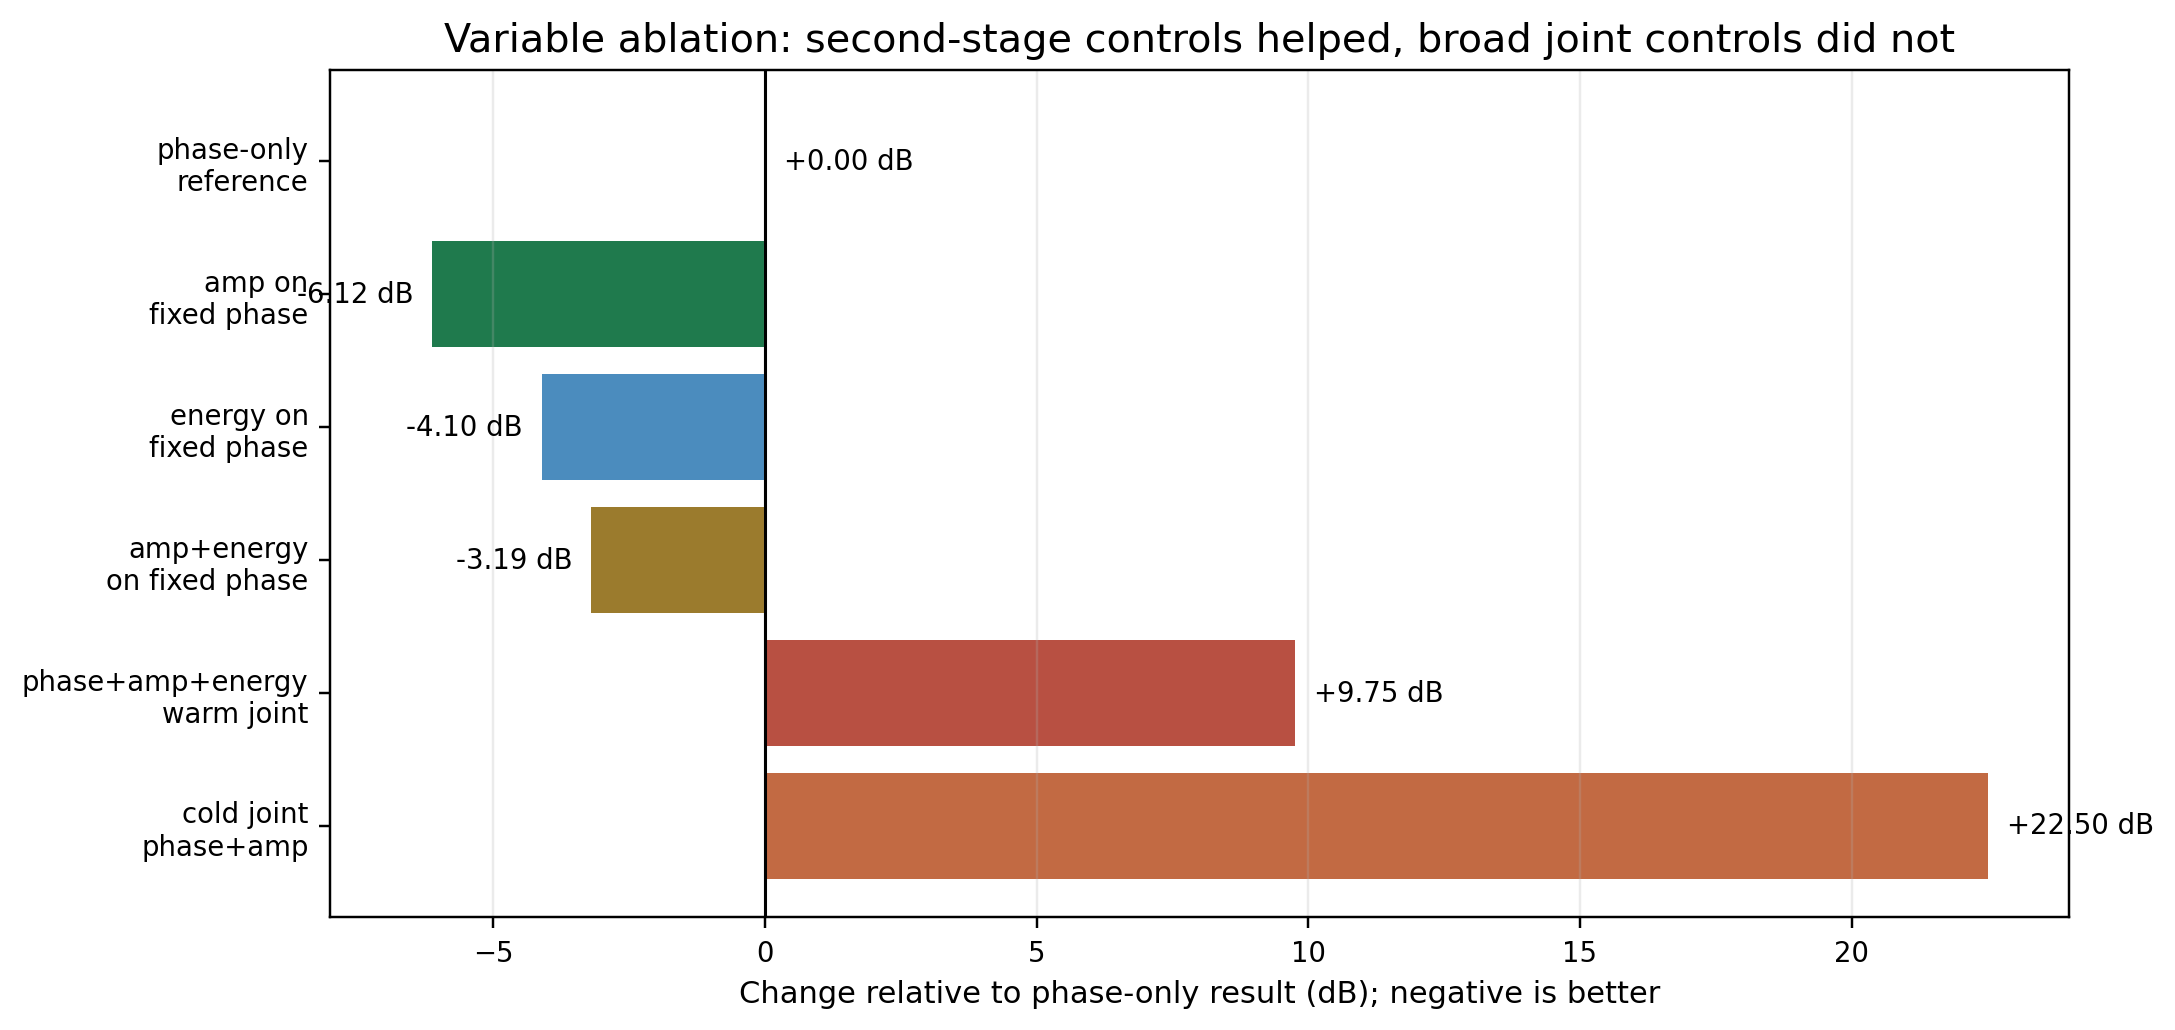
\includegraphics[width=0.95\linewidth]{figures/variable_ablation_summary.png}
\caption{The ablation result is not ``all extra variables help.'' It is specifically that small second-stage controls can help after the phase problem has already been solved.}
\end{figure}

\begin{figure}[H]
\centering
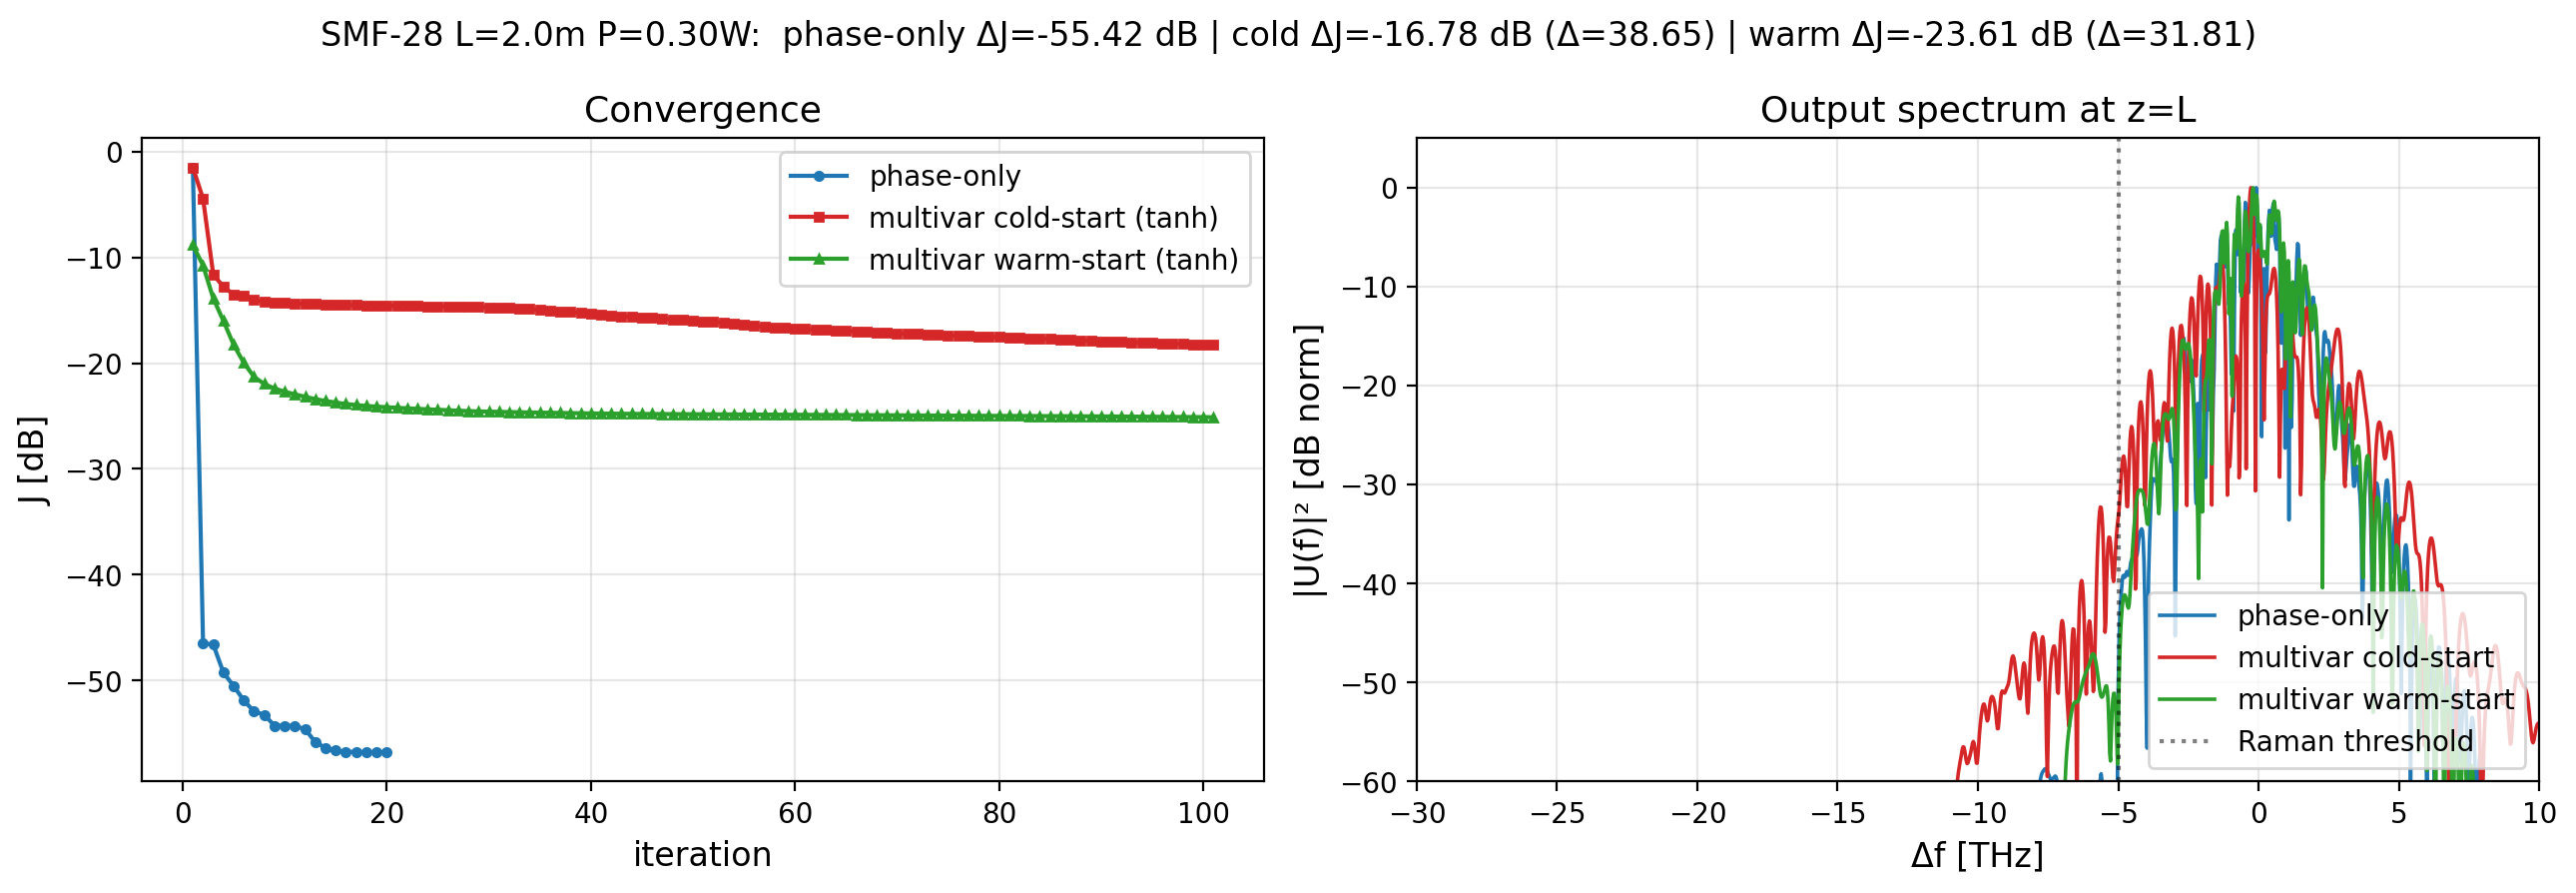
\includegraphics[width=0.92\linewidth]{figures/joint_controls_negative_result.png}
\caption{Earlier joint phase+amplitude runs underperformed the phase-only reference. This figure is kept because the negative result prevents overclaiming the multivariable lane.}
\end{figure}

\subsection{Amplitude-Bound Sweep}
\begin{figure}[H]
\centering
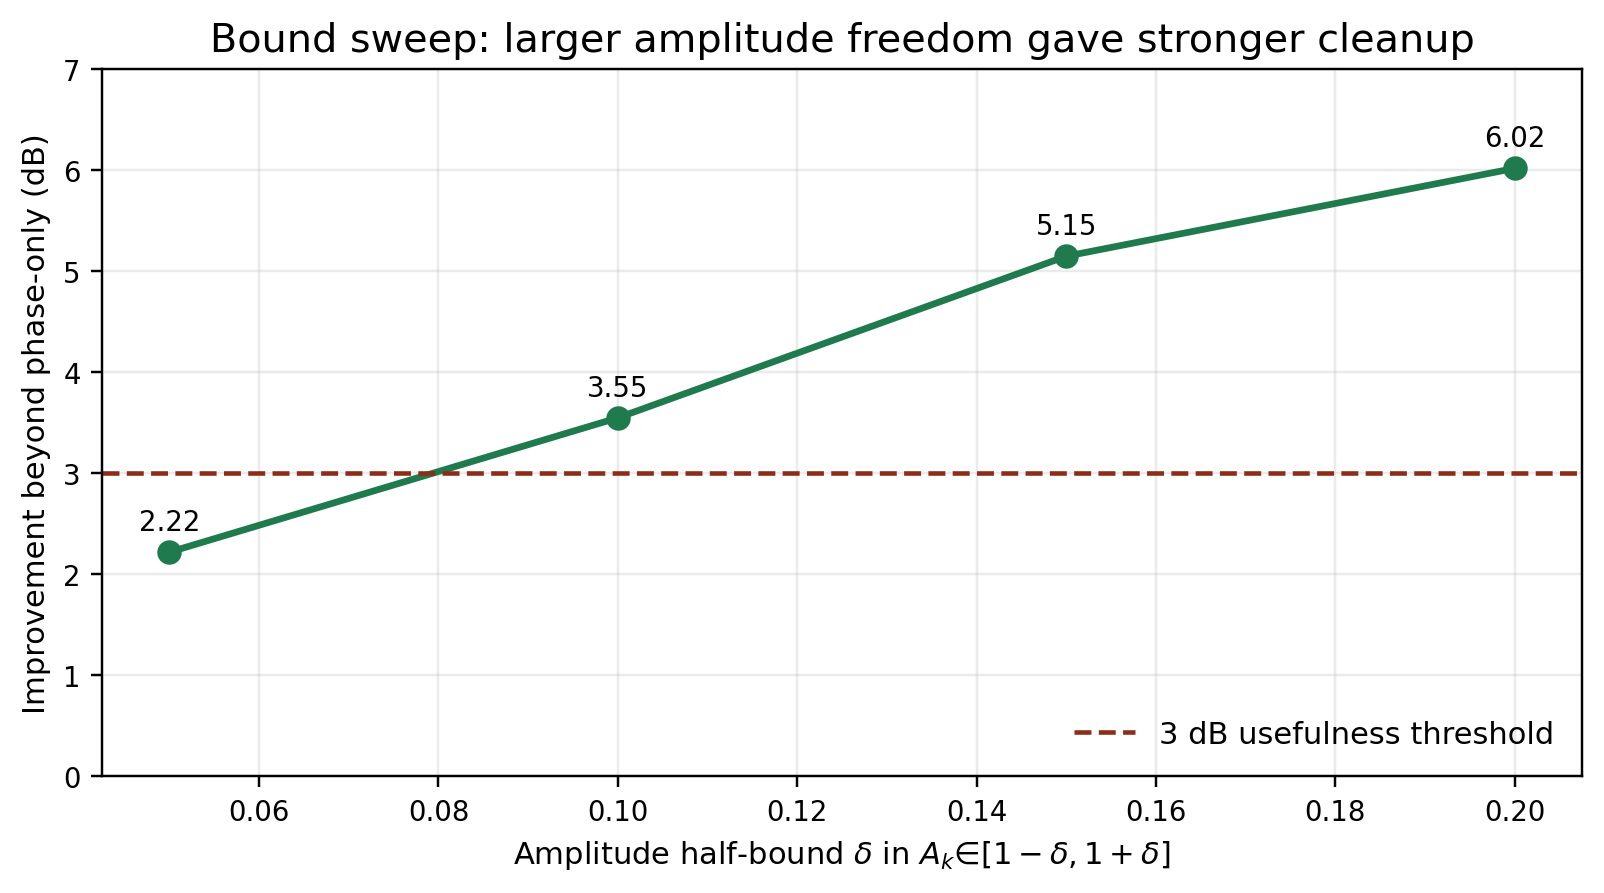
\includegraphics[width=0.76\linewidth]{figures/amplitude_bound_sweep.png}
\caption{Short canonical bound sweep. A small $\delta=0.05$ bound did not clear the 3 dB usefulness threshold; $\delta=0.10$ and larger did. The long $\delta=0.10$ ablation later reached $6.12$ dB but hit its iteration cap.}
\end{figure}

\begin{table}[H]
\centering
\small
\begin{tabular}{@{}rrrrr@{}}
\toprule
\textbf{Bound $\delta$} & \textbf{$J_{\mathrm{R}}$ dB} & \textbf{vs. phase-only} & \textbf{Iterations} & \textbf{Amplitude range} \\
\midrule
0.05 & $-43.01$ & $-2.22$ dB & 8 & $[0.950,1.050]$ \\
0.10 & $-44.34$ & $-3.55$ dB & 9 & $[0.908,1.090]$ \\
0.15 & $-45.94$ & $-5.15$ dB & 8 & $[0.855,1.149]$ \\
0.20 & $-46.82$ & $-6.02$ dB & 13 & $[0.805,1.199]$ \\
\bottomrule
\end{tabular}
\caption{Bound sweep for amplitude-on-fixed-phase refinement. Larger amplitude freedom helps in simulation, but it may also be harder to realize on a real shaper.}
\end{table}

\subsection{Local Robustness Check}
\begin{figure}[H]
\centering
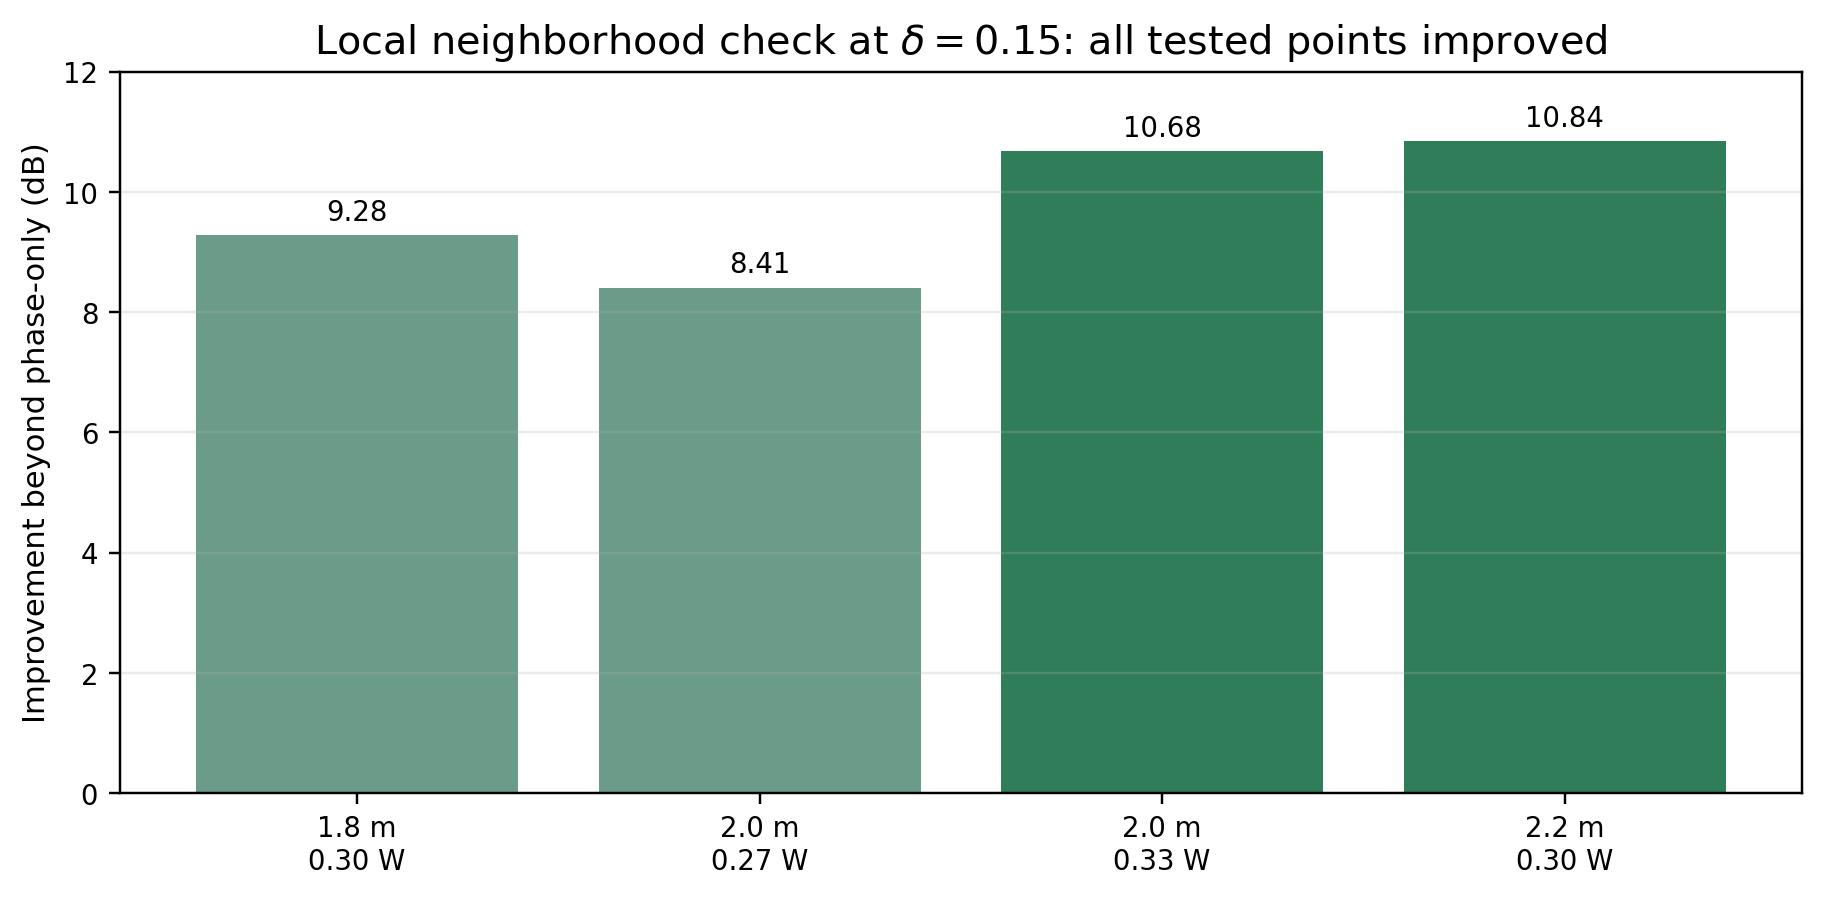
\includegraphics[width=0.80\linewidth]{figures/local_robustness_summary.png}
\caption{At $\delta=0.15$, nearby length/power points all showed amplitude-on-fixed-phase improvements larger than 8 dB. These runs hit 50 iterations, so the trend is more important than the exact last digit.}
\end{figure}

\begin{figure}[H]
\centering
\begin{minipage}{0.48\linewidth}
\centering
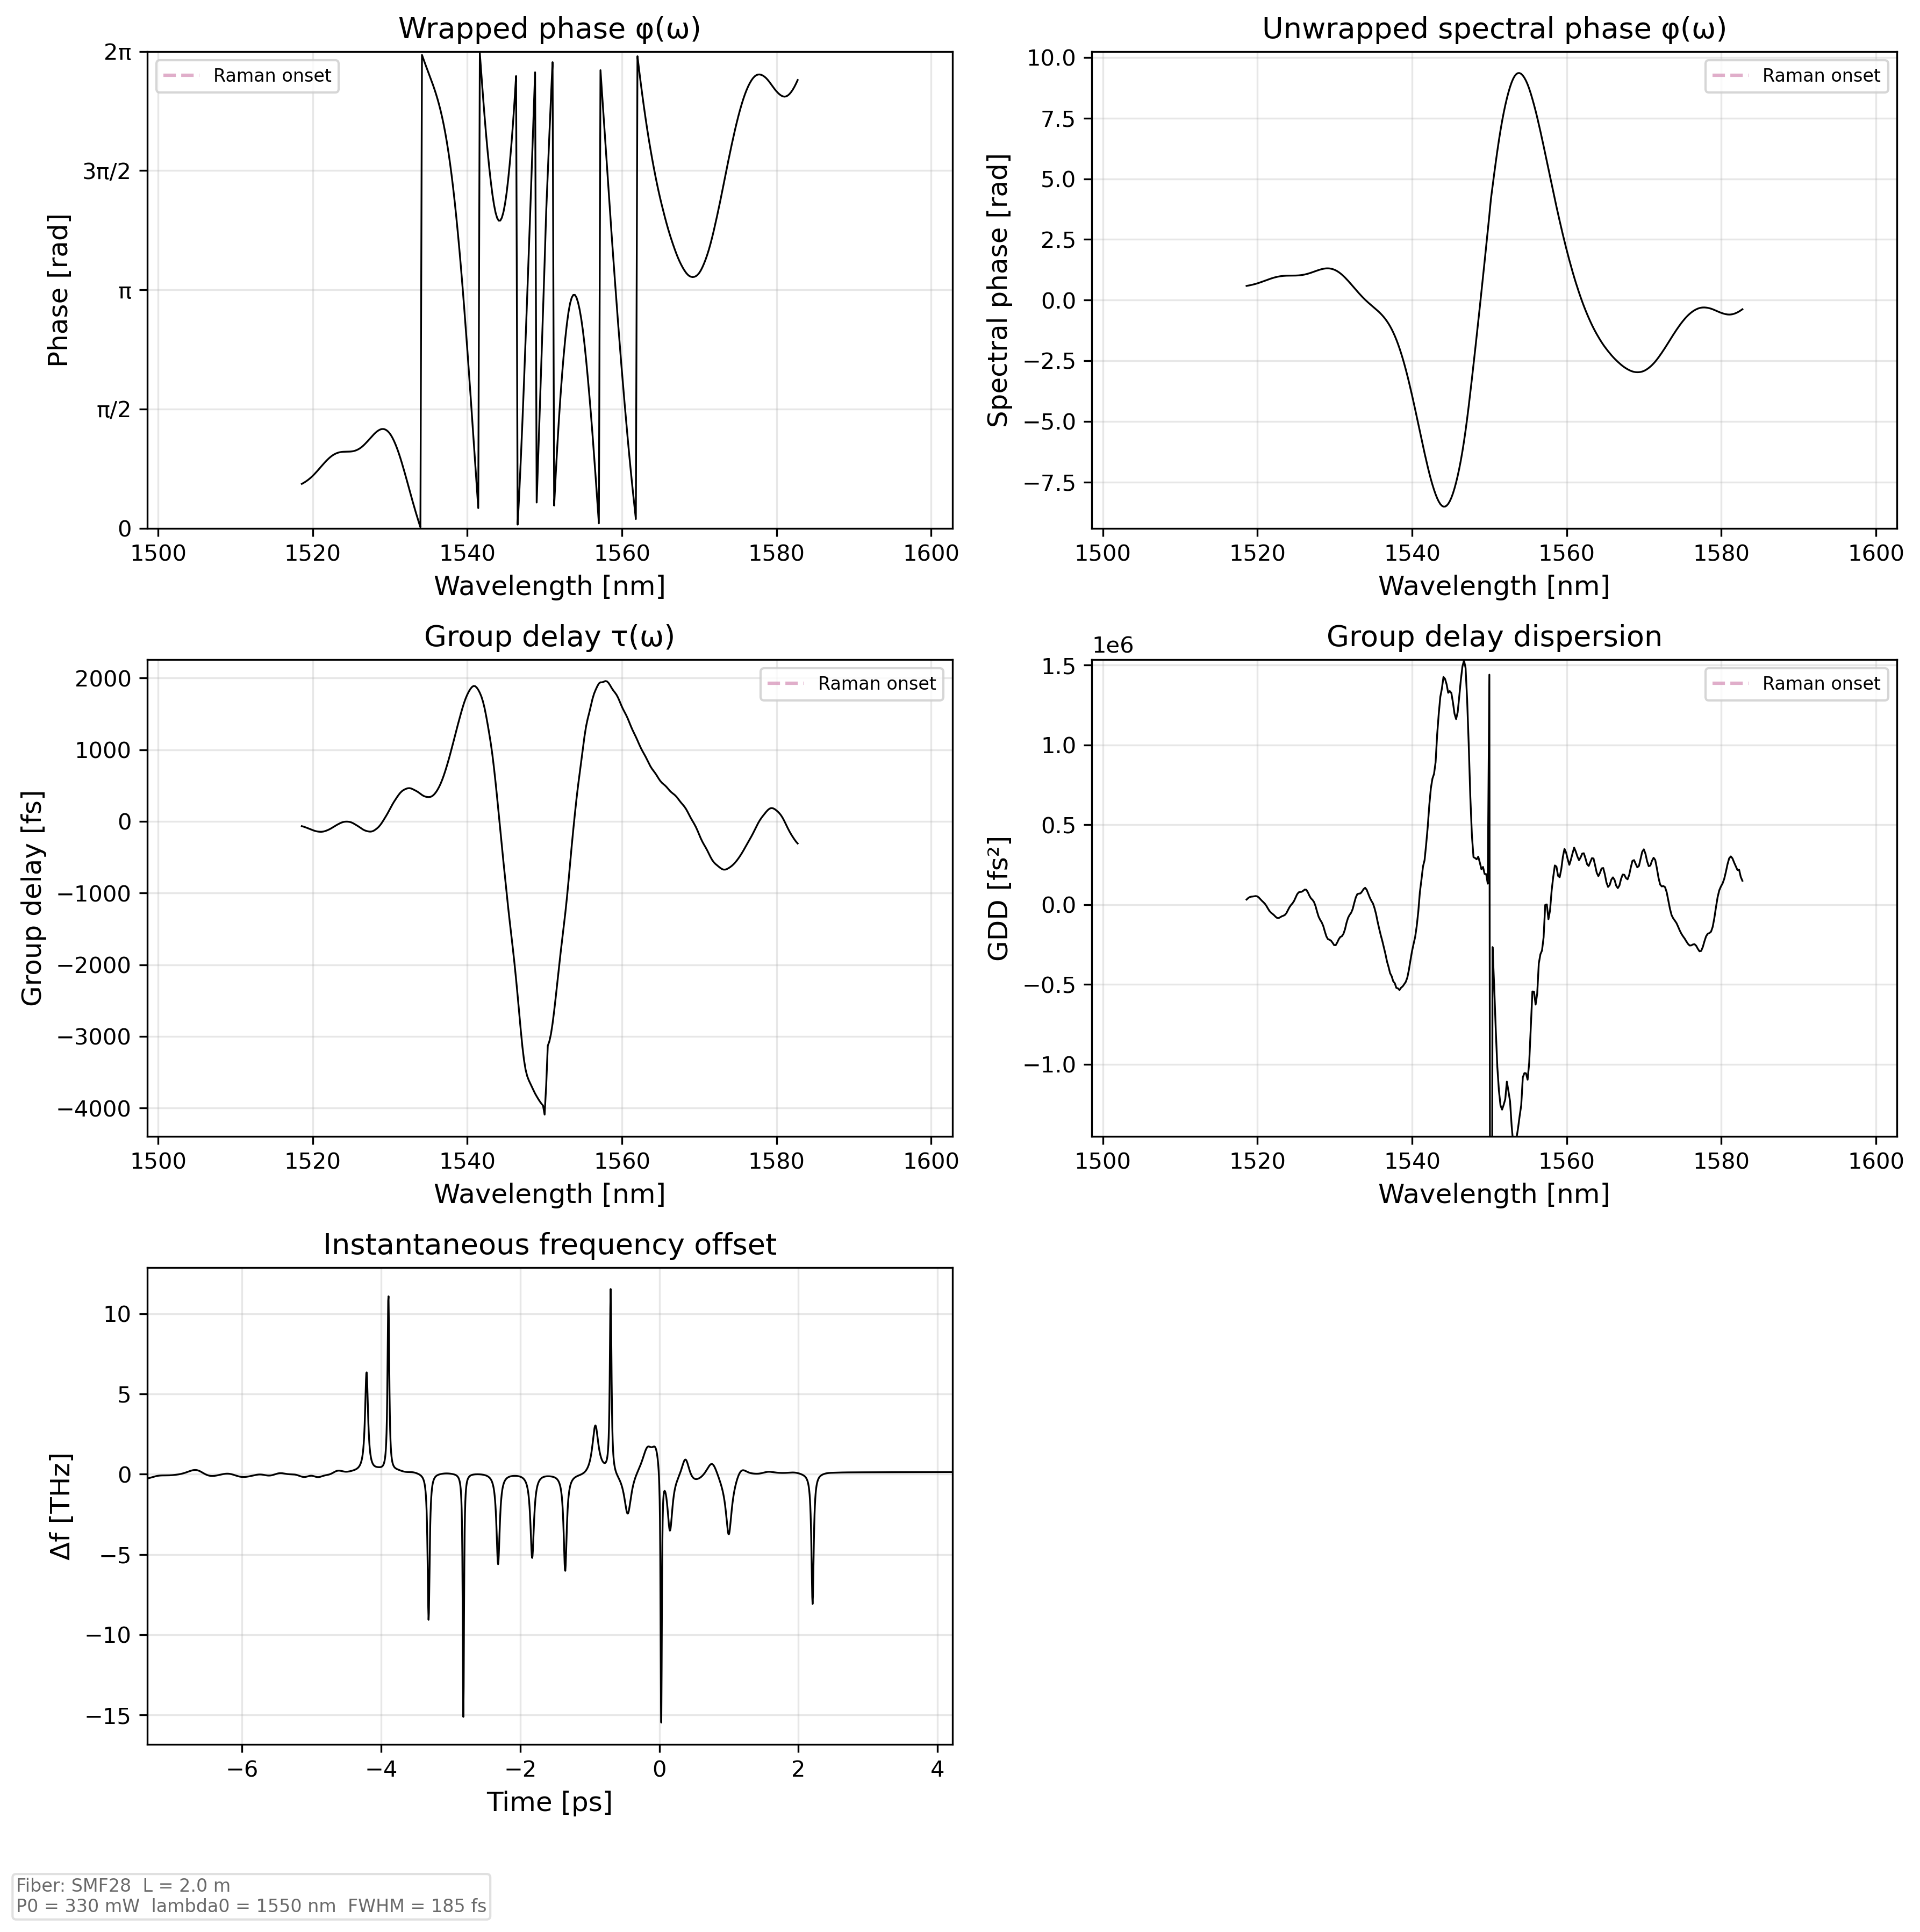
\includegraphics[width=\linewidth]{figures/local_best_phase_only_reference_phase_diagnostic.png}
\caption*{Local phase-only reference.}
\end{minipage}
\hfill
\begin{minipage}{0.48\linewidth}
\centering
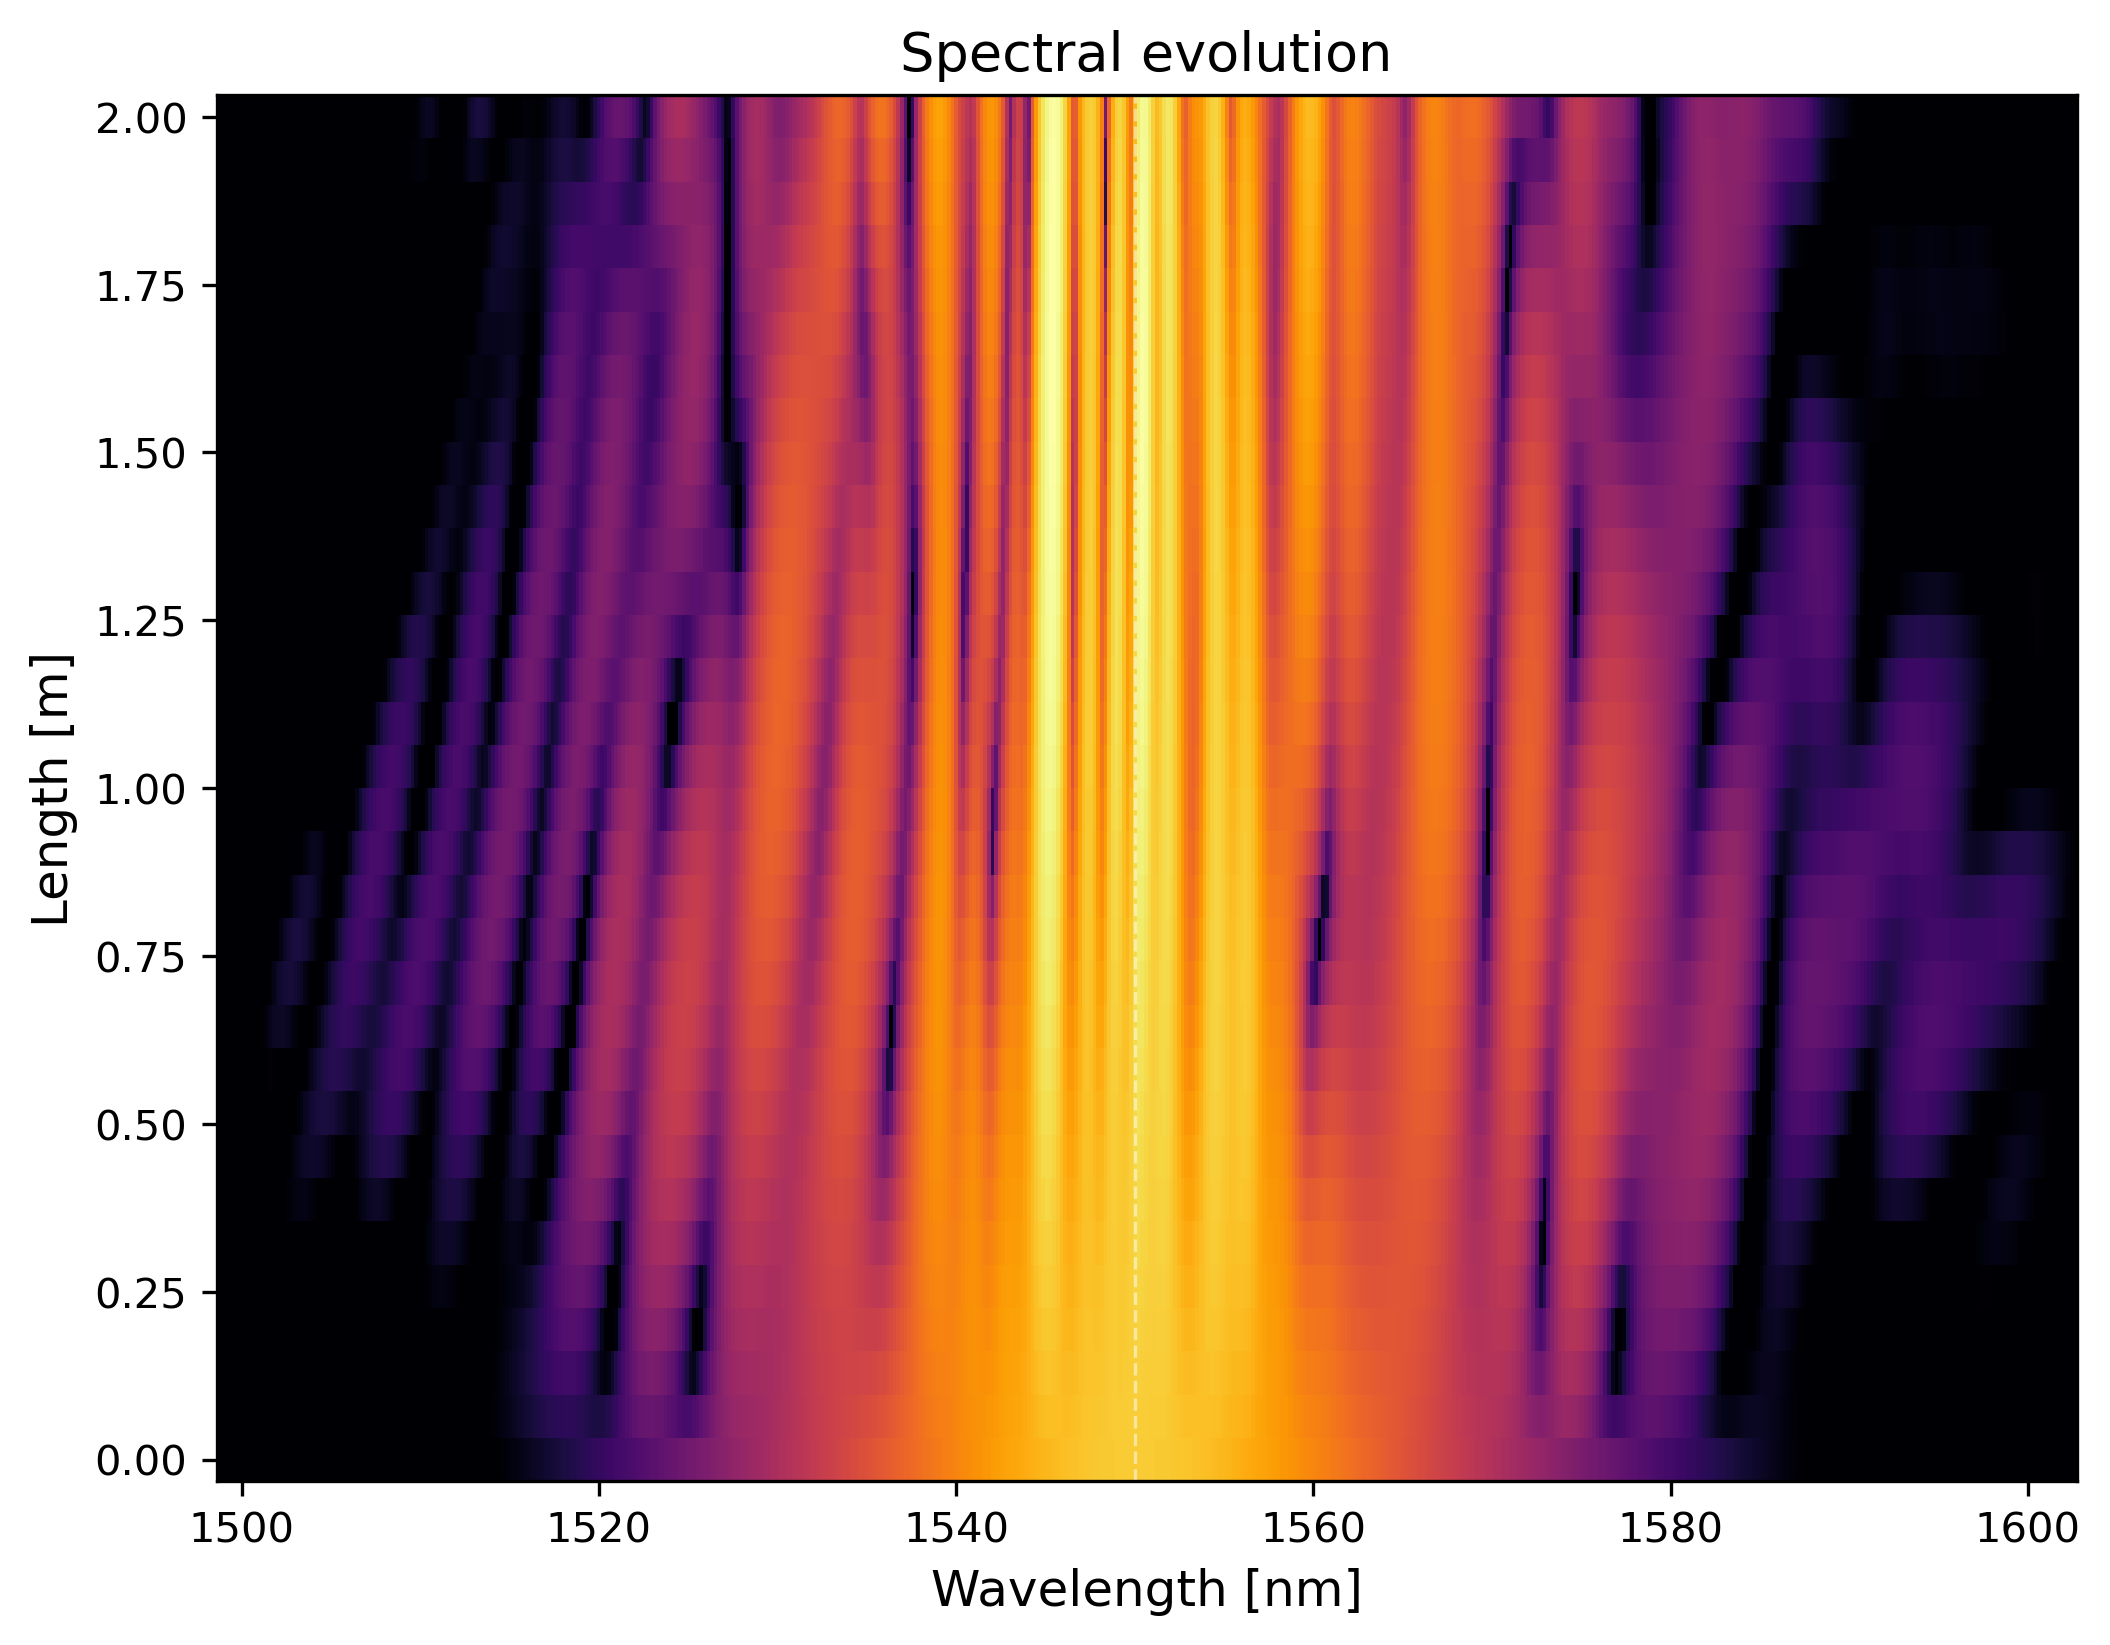
\includegraphics[width=\linewidth]{figures/local_best_phase_only_reference_evolution.png}
\caption*{Local phase-only heatmap.}
\end{minipage}
\vspace{0.7em}

\begin{minipage}{0.48\linewidth}
\centering
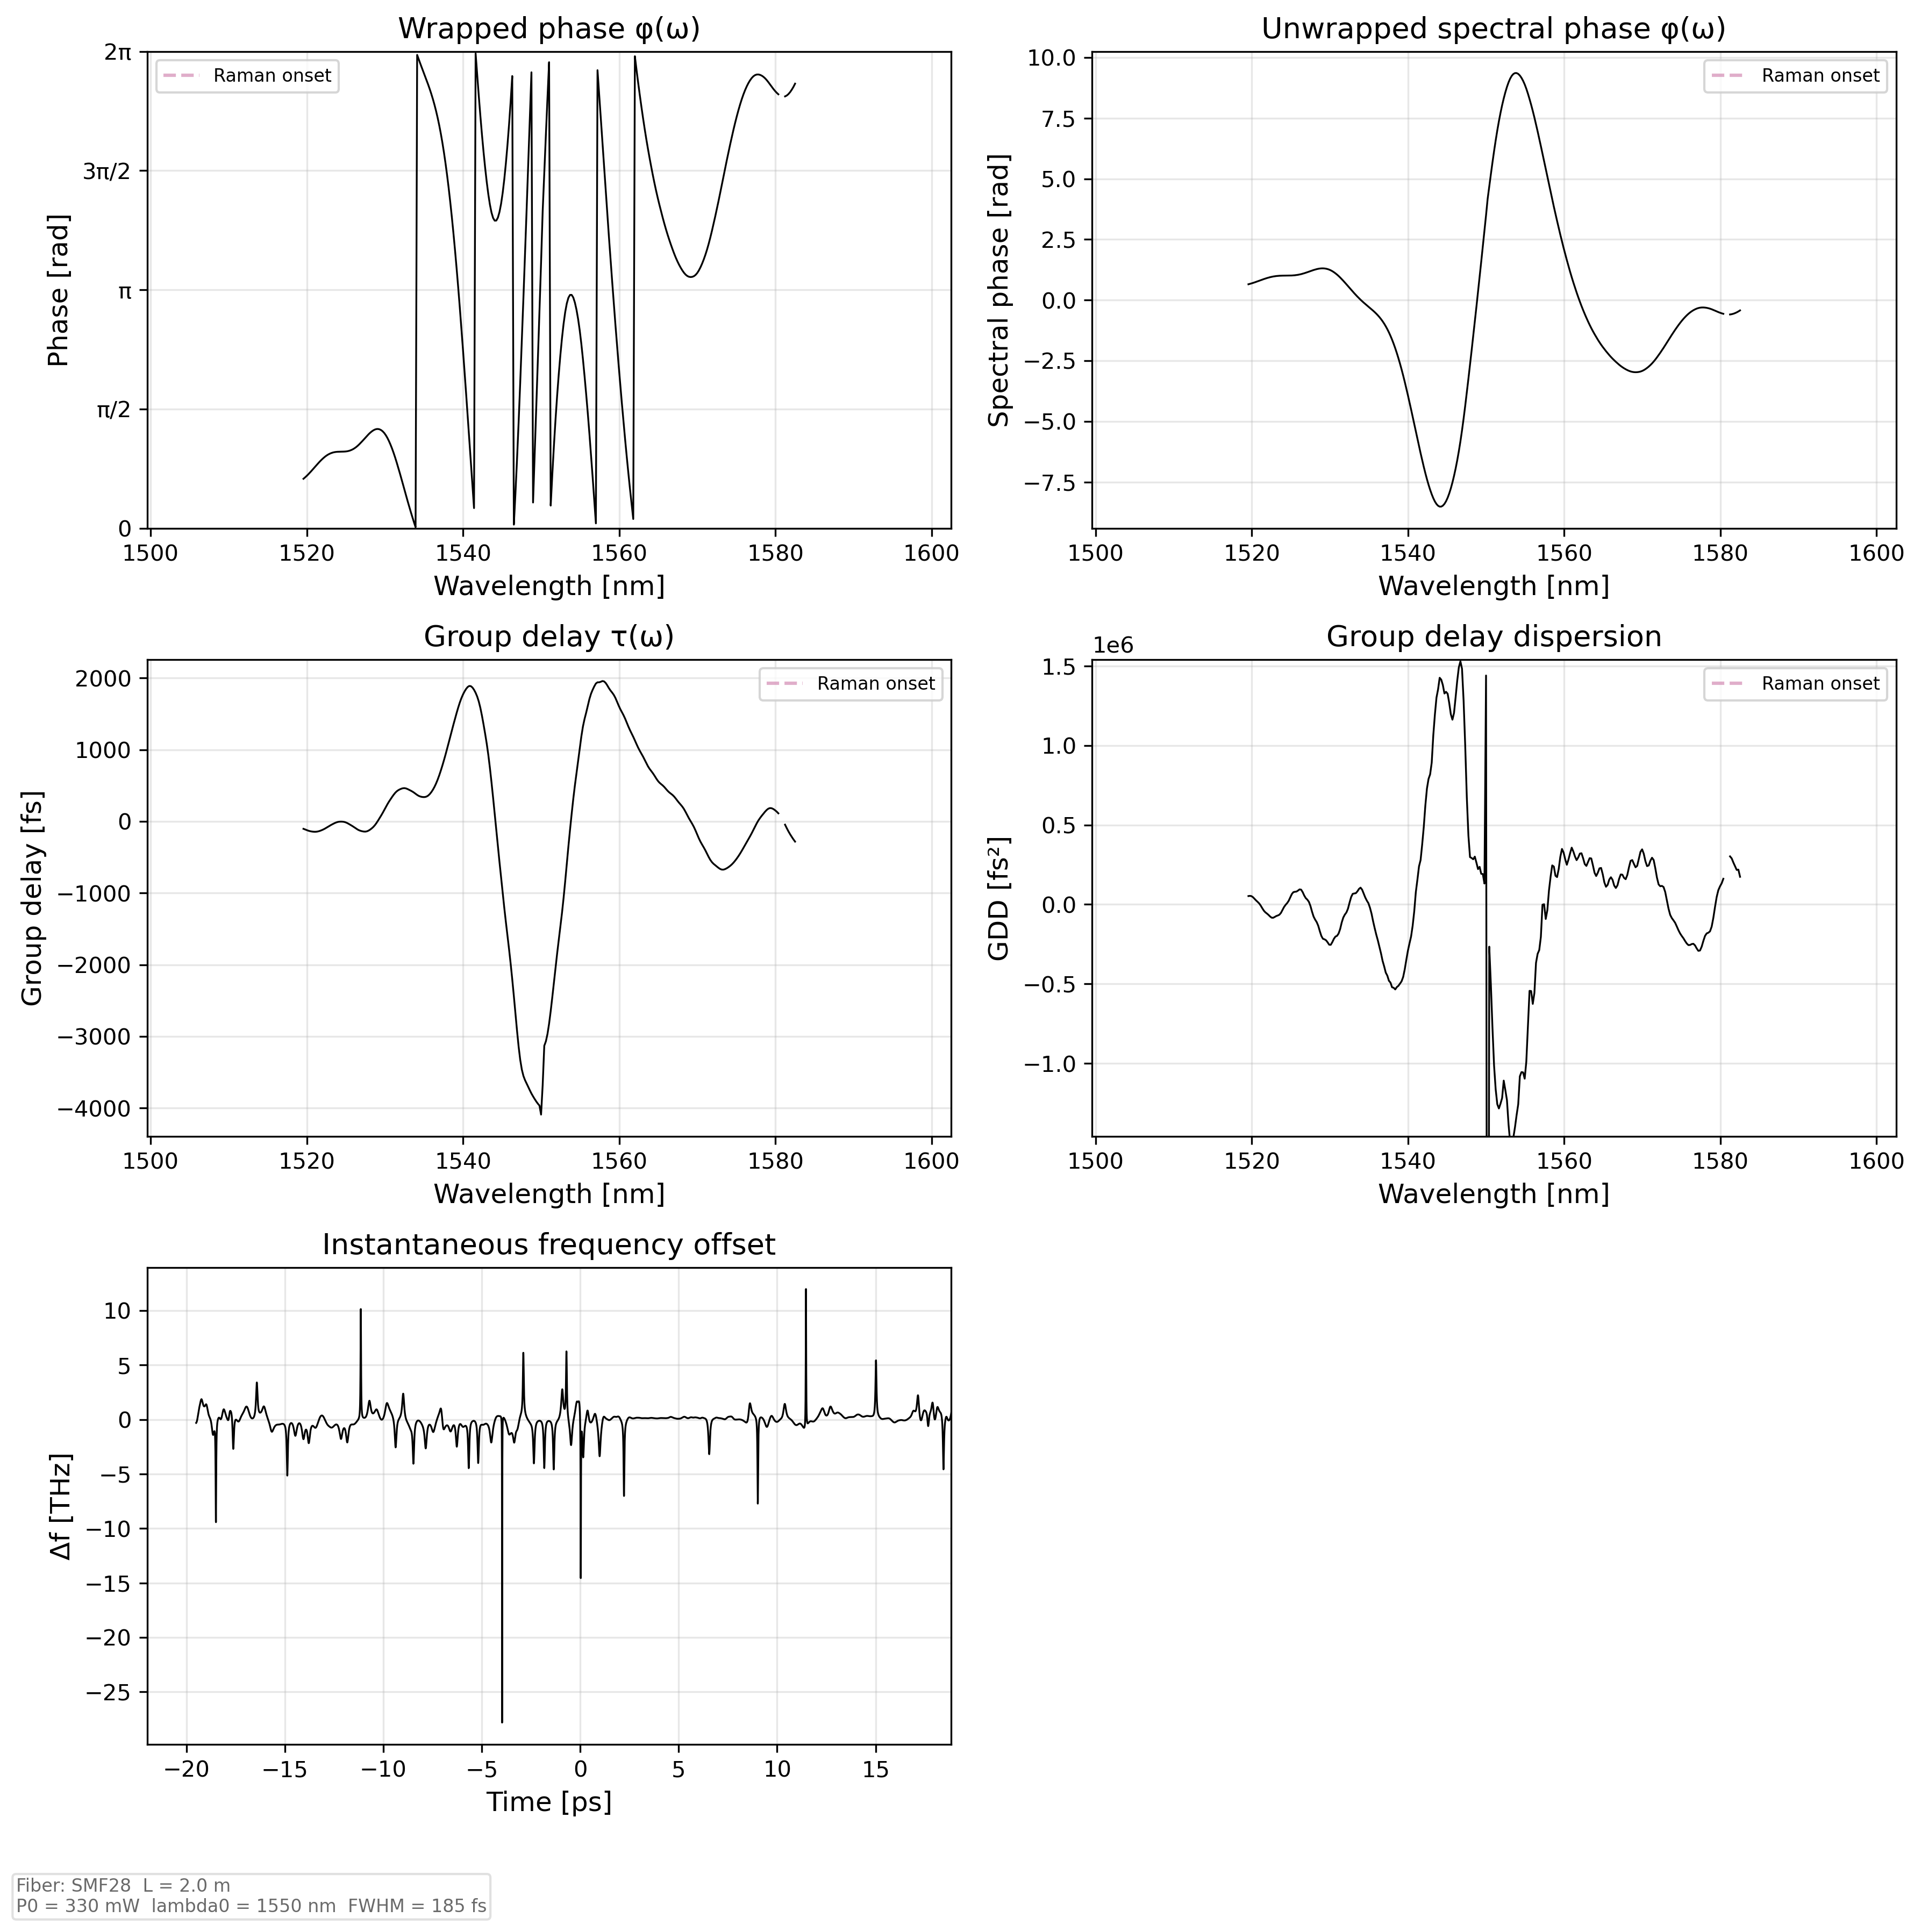
\includegraphics[width=\linewidth]{figures/local_best_amplitude_refinement_phase_diagnostic.png}
\caption*{Local amplitude-refined diagnostic.}
\end{minipage}
\hfill
\begin{minipage}{0.48\linewidth}
\centering
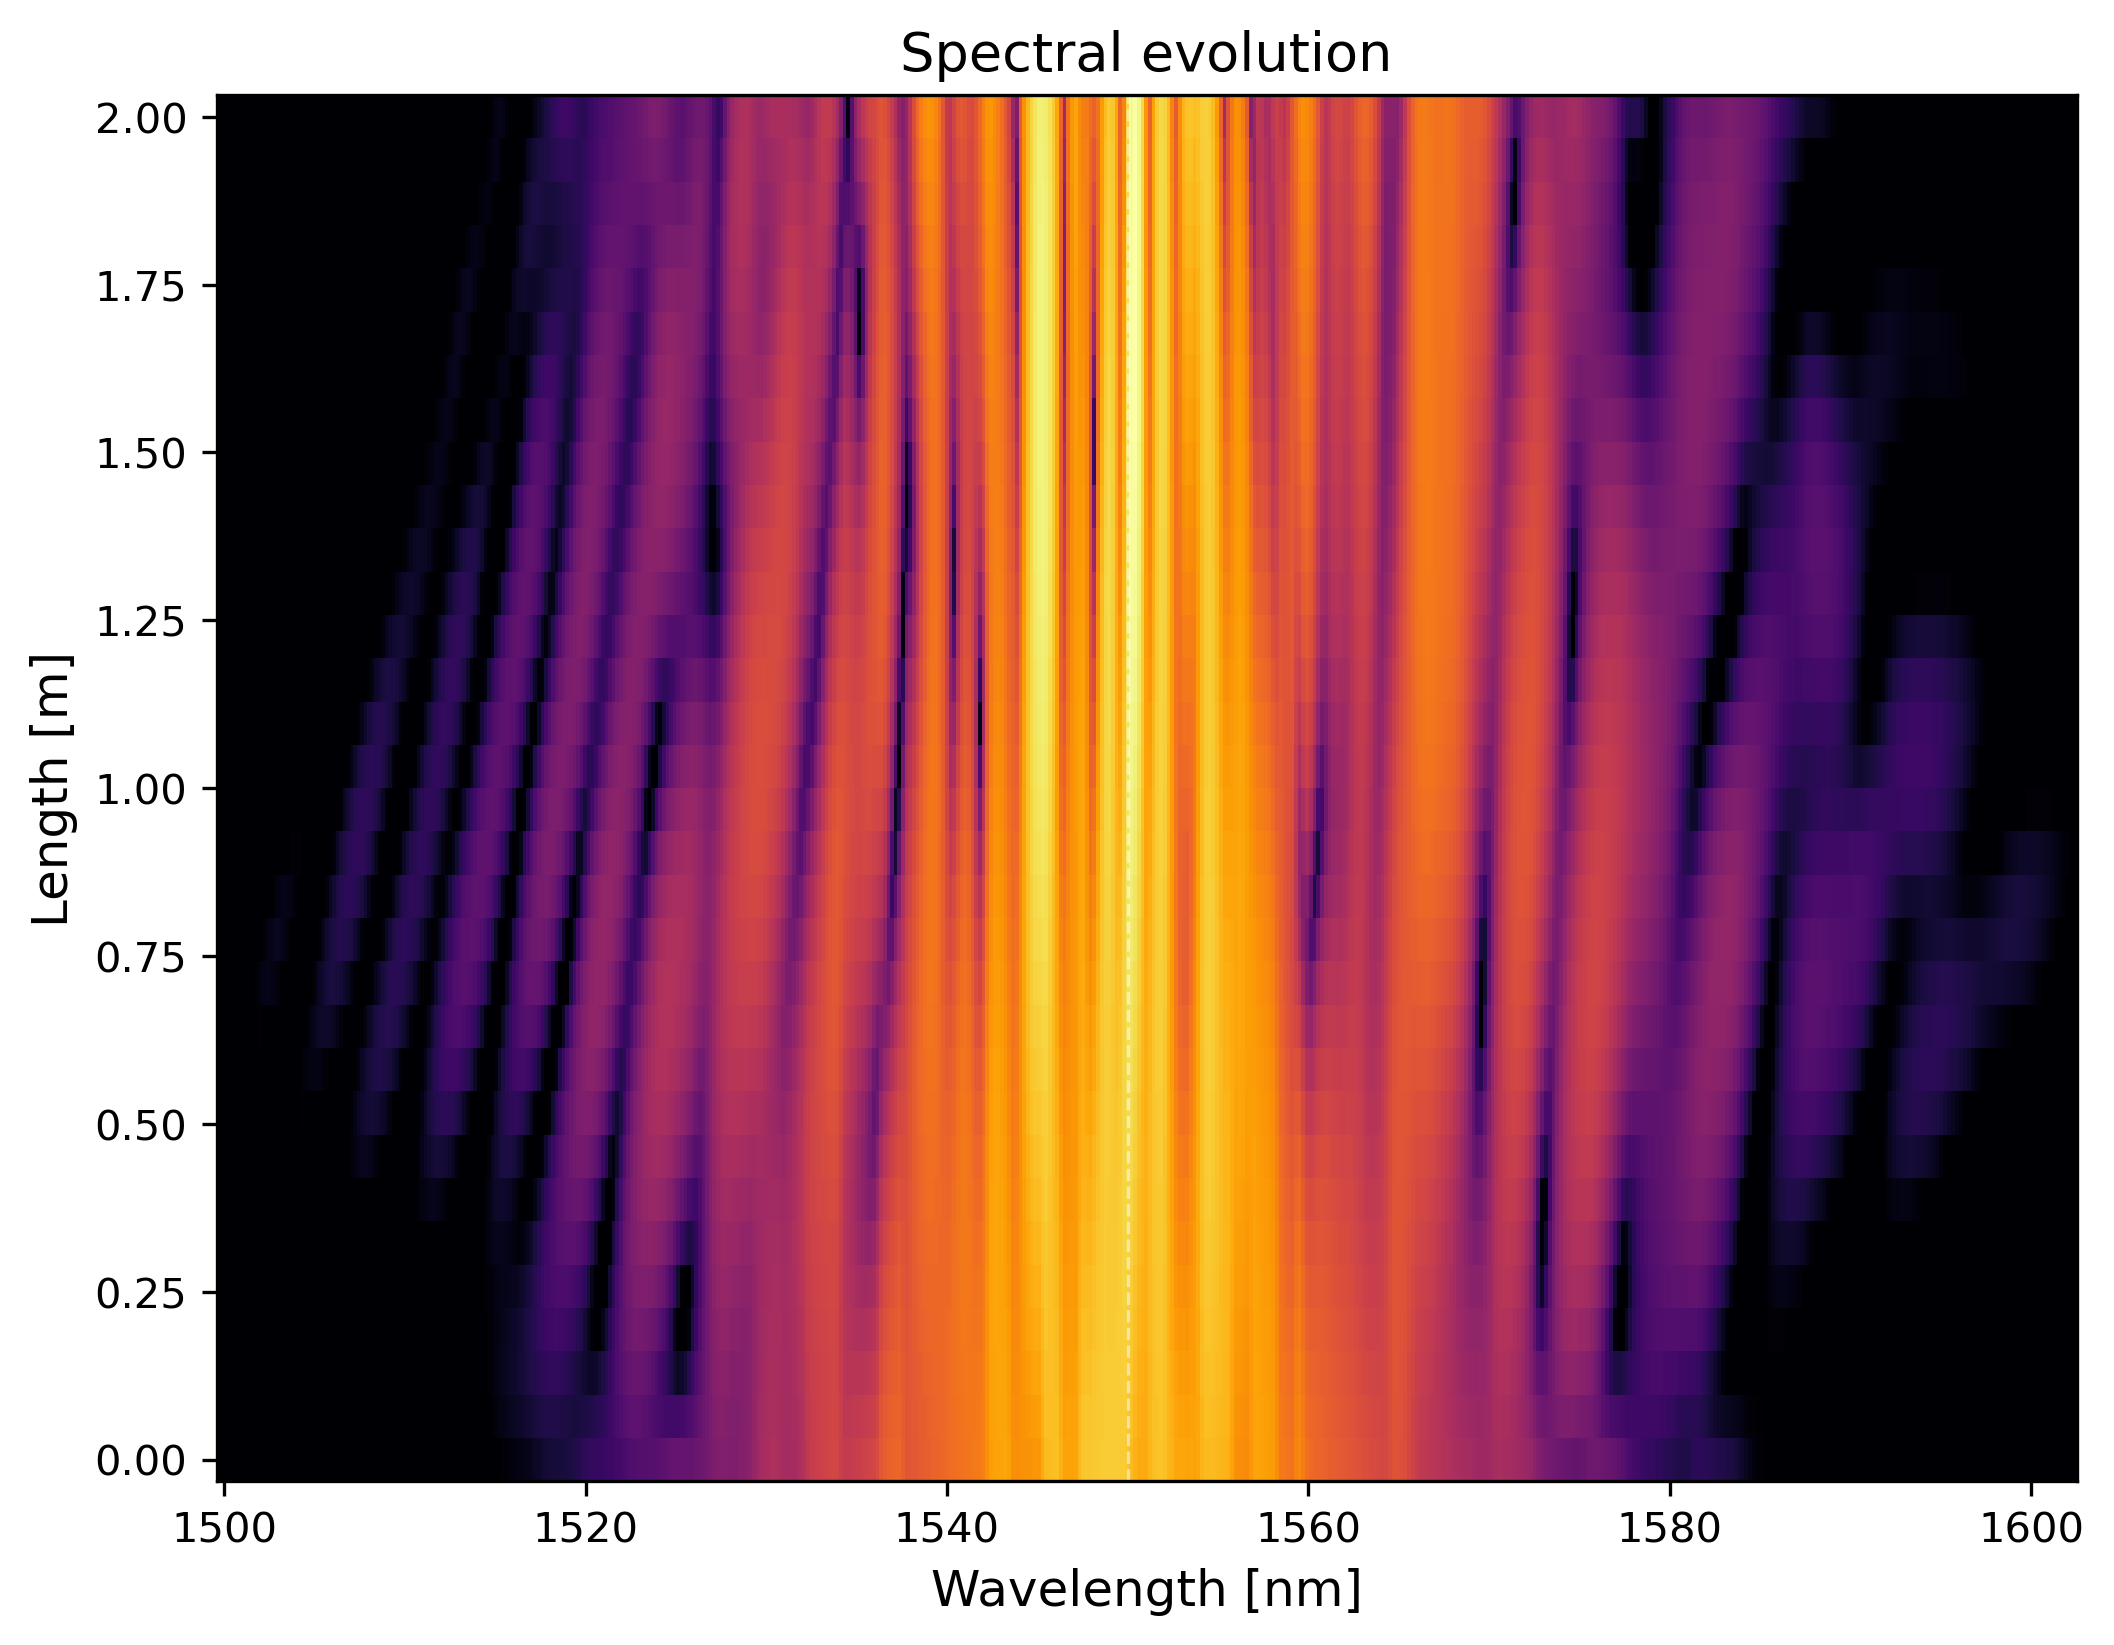
\includegraphics[width=\linewidth]{figures/local_best_amplitude_refinement_evolution.png}
\caption*{Local amplitude-refined heatmap.}
\end{minipage}
\caption{Representative local check at $L=2.0$ m and $P=0.33$ W. The phase-only reference was $-43.56$ dB and the amplitude-refined result was $-54.24$ dB, a $10.68$ dB improvement.}
\end{figure}

\FloatBarrier

\section{Interpretation}
The most important lesson is that dimensionality is not free. Adding amplitude and energy variables creates a much larger landscape, and the optimizer can waste effort undoing phase structure that already works. The staged method avoids that by preserving the phase-only solution and giving the second stage a smaller, more local job.

The amplitude result is also physically interpretable. Phase shaping can move energy in time and frequency through propagation, but after a phase-only optimum there may still be residual spectral regions that seed Raman leakage. Bounded amplitude shaping can slightly suppress or emphasize those regions before propagation. In the current results, amplitude values often press against their allowed bounds, which means the bound is an active modeling choice rather than a harmless detail.

\section{Presentation Capsule}
If this note becomes one slide in a presentation, the clean message is:
\begin{itemize}
    \item Phase-only shaping is still the main baseline.
    \item Full joint optimization was a negative result.
    \item A second-stage amplitude correction after phase-only shaping gave an additional $3.5$--$6.1$ dB at the canonical point and larger improvements in a nearby $\delta=0.15$ check.
    \item The result is promising but not lab-final because amplitude masks and energy retuning need calibration and fairness checks.
\end{itemize}

\section{Limitations and Missing Evidence}
\begin{itemize}
    \item \textbf{Hardware realism.} The simulated amplitude mask allows $\Avar_k>1$. A loss-only shaper cannot create gain, so lab transfer needs normalization or calibration.
    \item \textbf{Iteration caps.} Several strong runs hit a 50-iteration cap. They are valid evidence that the method helps, but not proof of final convergence.
    \item \textbf{Energy fairness.} Energy-only improvements may partly reflect retuning launch power. This is useful physics information but not automatically a fair fixed-power comparison.
    \item \textbf{Mode coefficients.} Mode-coordinate optimization is not complete; current code strips the mode-coefficient option and warns.
    \item \textbf{Parameter coverage.} The strongest evidence is near the SMF-28 2 m, 0.3 W setting. Wider fiber, power, and pulse-grid sweeps would be needed before making universal claims.
    \item \textbf{Lab handoff.} The amplitude-aware export path exists, but it still needs real shaper transfer-function validation.
\end{itemize}

\section{Reproduction Capsule}
Light local verification commands:
\begin{verbatim}
julia -t auto --project=. scripts/dev/smoke/test_multivar_unit.jl
julia -t auto --project=. scripts/dev/smoke/test_multivar_gradients.jl
\end{verbatim}

Dry-run the optional two-stage workflow:
\begin{verbatim}
julia -t auto --project=. scripts/canonical/refine_amp_on_phase.jl --dry-run
\end{verbatim}

Run a new amplitude-on-phase refinement, preferably on the heavy compute machine for full-resolution work:
\begin{verbatim}
julia -t auto --project=. scripts/canonical/refine_amp_on_phase.jl \
  --tag my_amp_refinement --L 2.0 --P 0.30 \
  --phase-iter 50 --amp-iter 60 --delta-bound 0.10 --export
\end{verbatim}

Expected closeout artifacts are an \texttt{amp\_on\_phase\_summary.md}, an \texttt{amp\_on\_phase\_result.jld2}, an optional \texttt{export\_handoff/} directory, and the standard image set:
\begin{itemize}
    \item phase diagnostic,
    \item optimized propagation heatmap,
    \item unshaped-control propagation heatmap,
    \item SLM/export metadata where applicable.
\end{itemize}

\section{Source Notes}
\begin{itemize}
    \item The fiber-propagation context follows generalized nonlinear fiber optics models; see Agrawal's \noteurl{https://www.sciencedirect.com/book/monograph/9780128170427/nonlinear-fiber-optics}{\emph{Nonlinear Fiber Optics}}.
    \item The interaction-picture numerical framing is consistent with Hult's RK4IP method for generalized nonlinear Schrödinger propagation: \noteurl{https://opg.optica.org/abstract.cfm?URI=JLT-25-12-3770}{Journal of Lightwave Technology 25(12), 3770--3775}.
    \item The optimization vocabulary for model agreement and trust-region thinking follows Nocedal and Wright's \emph{Numerical Optimization}; the actual/predicted-reduction ratio is summarized in many course notes and in the textbook discussion of trust-region methods.\footnote{\noteurl{https://link.springer.com/book/10.1007/978-0-387-40065-5}{Nocedal and Wright, \emph{Numerical Optimization}, Springer}.}
\end{itemize}

\end{document}
